%----------------------------------------------------------------------------
% Magic Maintainer's Manual #2
%----------------------------------------------------------------------------

\NeedsTeXFormat{LaTeX2e}[1994/12/01]
\documentclass[letterpaper,twoside,12pt]{article}
\usepackage{epsfig,times,pifont}

\setlength{\textwidth}{8.5in}
\addtolength{\textwidth}{-2.0in}
\setlength{\textheight}{11.0in}
\addtolength{\textheight}{-2.0in}
\setlength{\oddsidemargin}{0in}
\setlength{\evensidemargin}{0pt}
\setlength{\topmargin}{-0.5in}
\setlength{\headheight}{0.2in}
\setlength{\headsep}{0.3in}
\setlength{\topskip}{0pt}

\def\hinch{\hspace*{0.5in}}
\def\starti{\begin{center}\begin{tabbing}\hinch\=\hinch\=\hinch\=\hinch\=\kill}
\def\endi{\end{tabbing}\end{center}}
\def\ii{\>\>\>}
\def\I{\hinch}
\def\II{\I\I}
\def\vns{\vspace*{-0.05in}}
\def\mytitle{Magic Maintainer's Manual \#2: The Technology File}
\def\q{\special{ps:(") show}\hspace*{0.6em}}
\def\grt{\hspace*{0.3em}\special{ps:(>) show}\hspace*{0.3em}}
\def\bk{\special{ps:/bksp 2 string def bksp 0 92 put bksp show}\hspace*{0.4em}}
\def\vbar{$|$}

\newcommand{\micro}{\Pifont{psy}m}
\newcommand{\ohms}{\Pifont{psy}W}

%----------------------------------------------------------------------------

\begin{document}

\makeatletter
\newcommand{\ps@magic}{%
	\renewcommand{\@oddhead}{\mytitle\hfil\today}%
	\renewcommand{\@evenhead}{\today\hfil\mytitle}%
	\renewcommand{\@evenfoot}{\hfil\textrm{--{\thepage}--}\hfil}%
	\renewcommand{\@oddfoot}{\@evenfoot}}
\newcommand{\ps@mplain}{%
	\renewcommand{\@oddhead}{}%
	\renewcommand{\@evenhead}{}%
	\renewcommand{\@evenfoot}{\hfil\textrm{--{\thepage}--}\hfil}%
	\renewcommand{\@oddfoot}{\@evenfoot}}
\makeatother
\pagestyle{magic}
\thispagestyle{mplain}


\begin{center}
  {\bfseries \Large \mytitle} \\
  \vspace*{0.5in}
  {\itshape Walter Scott} \\
  \vspace*{0.25in}
   Special Studies Program \\
   Lawrence Livermore National Laboratory \\
   P.O. Box 808, L-270 \\
   Livermore, CA  94550 \\
  \vspace*{0.25in}
  {\itshape John Ousterhout} \\
  \vspace*{0.25in}
   Computer Science Division \\
   Electrical Engineering and Computer Sciences \\
   University of California \\
   Berkeley, CA  94720 \\
  \vspace*{0.25in}
  {\itshape (Updated by others, too.)} \\
  \vspace*{0.25in}
  This manual corresponds to Magic version 7.4
  and technology format 30
\end{center}
\vspace*{0.25in}

{\noindent\bfseries\large Tutorials to read first:}
\starti
   \> Magic Tutorial \#1: Getting Started \\
   \> Magic Tutorial \#2: Basic Painting and Selection \\
   \> Magic Tutorial \#6: Design-Rule Checking \\
   \> Magic Tutorial \#8: Circuit Extraction \\
   \> Magic Tutorial \#9: Format Conversion for CIF and Calma
\endi
\noindent You should also read at least the first, and probably all four,
of the papers on Magic that appeared in the {\itshape ACM IEEE 21st
Design Automation Conference}, and the paper ``Magic's Circuit Extractor'',
which appeared in the {\itshape ACM IEEE 22nd Design
Automation Conference}.  The overview paper from the
DAC was also reprinted in {\itshape IEEE Design and Test} magazine in
the February 1985 issue.
The circuit extractor paper also appeared in the
February 1986 issue of {\itshape IEEE Design and Test} magazine. 

{\noindent\bfseries\large Commands introduced in this manual:}
\starti
   \> path
   \> tech
   \> *watch
\endi

{\noindent\bfseries\large Macros introduced in this manual:}

\starti
   \> {\itshape (None)}
\endi

{\noindent\bfseries\large Changes since Magic version 7.2:}
\begin{itemize}
\item Support for stacked contacts.
\item ``variants'' option for the cifinput, cifoutput, and extract
	sections, allowing an efficient description of different
	styles having minor variations.
\item Supports names for layer drawing styles in addition to the usual
	numbers.
\item Section name {\bfseries images} duplicates the {\bfseries contacts}
	section, allowing a less-restrictive definition of images that
	exist, like contacts, on multiple planes.
\item Support for multi-line technology descriptions.
\item ``include'' statement to divide technology files into parts.
\item ``alias'' statements to replace the original cpp-style macros
\item Support for {\itshape angstroms} in the scalefactor line of
	cifinput and cifoutput.
\item Additional DRC types ``surround'', ``overhang'', and ``rect\_only''.
\item Additional cifoutput operators ``slots'' and ``bloat-all''.
\item Additional cifoutput statement ``render'' for 3-D information
\item Asterisk syntax for layers that expands to the layer and all of
	the contacts containing that layer as a residue.
\item The technology file syntax for the PNM format was changed in
	magic 7.3.56, and the {\bfseries plot pnm} command will
	use a default style derived from the layout styles if no
	section is present in the technology file.
\end{itemize}

{\noindent\bfseries\large Changes since Magic version 6.5:}
\begin{itemize}
\item Moved technology format from the filename to the ``tech'' section
\item Added subdirectory searching to the path search for technology files.
\item Support for technology file re-loading after Magic starts up, and
	support for re-loading of individual sections of the technology
	file.
\item Scalefactors can now be any number whatsoever, for both CIF and GDS.
	For example, a scalefactor of 6.5 corresponds to a 0.13 micron
	process.
\item A parameter {\itshape nanometers} has been added to the scalefactor
	specification for both cifinput and cifoutput sections.  This
	parameter declares that all numbers in the style description are
	in nanometers instead of centimicrons.
\item The {\itshape calmaonly} parameter to the scalefactor specification is
	deprecated (ignored if found).
\item The scale reducer parameter is deprecated (generated automatically,
	and ignored if found in the techfile).
\item The magic grid spacing is no longer assumed to be equal to the process
	lambda.  It may be rescaled with the ``scalegrid'' command, and CIF
	and Calma reads may alter the value of magic units per lambda.
\item Support for PNM and PostScript graphics in the ``plot'' section.
\item Full support for bipolar junction transistors, capacitors, and
	resistors with the ``extract'' section keyword ``device''
\item Support for three-dimensional modeling and geometry extraction
\item Support for the DRC widespacing rule
\item Handling of contacts in the extraction section is capable of
	matching the CIF output section by specifying border, size,
	and spacing.
\end{itemize}

\vspace*{0.25in}
\section{Introduction}

Magic is a technology-independent layout editor.
All technology-specific information comes from a
{\itshape technology file}.  This file includes such information
as layer types used, electrical connectivity between types,
design rules, rules for mask generation, and rules for
extracting netlists for circuit simulation.

This manual describes the use, contents, and syntax of Magic's
technology file format, and gives hints for building a new one or
(more typically) rewriting an existing one for a new fabrication
process.  References to specific files in the Magic distribution
assume that your current working directory is the Magic source
top-level directory.

\section{Downloads and Installation}

Typically, there is a different technology file for each fabrication
process supported by Magic.  Scalable technologies, which are
(within limits) independent of feature size, will typically have
one technology file for all processes supporting the same set of
lambda-based (scalable) DRC rules.
That said, modern technologies (post-1980's, more or less) tend to
be more restrictive in their design rules, and consequently not
scalable.  This is particularly true of processes which push the
envelope on feature sizes.  

The Magic source distribution
is packaged with a ``standard'' set of scalable SCMOS rules, which
is the technology loaded by default.  Default settings are for
1\,{\micro}m technology, which is out of date.  However, the
variety and availability of processes means that the ``definitive''
set of technology files is prohibitively large to be included
with the Magic source.  In addition, process refinements generally
require technology file updates on a regular basis.  Because of
this, the basic collection of technology files is handled by the
MOSIS foundation, not by the Magic development team.  This
collection represents all processes which are available for
fabriction through the MOSIS foundation.  Most other vendors have
proprietary process specifications, requiring tool maintainers to
write their own technology files or modify an existing one to
match the proprietary process.

The standard technology file set can be downloaded from an FTP
server at the MOSIS foundation.  These files are regularly
updated, but there is usually a symbolic link called ``current''
to the most recent stable revision.  The download URL is the
following:

\starti
  \> {\ttfamily\bfseries ftp://ftp.mosis.edu/pub/sondeen/magic/new/beta/current.tar.gz}
\endi

Assuming that the install destination for magic is
{\bfseries /usr/local}, this file should be put either in {\bfseries
/usr/local/lib/magic/sys} or (preferably) in {\bfseries
/usr/local/lib/magic/sys/current}.  Other destinations may
be used, if the system search path is appropriately specified
on startup (see Section~\ref{commandline}, below).

The technology file collection is in tarred, gzipped format,
and should be installed with the following commands:

\starti
  \ii {\ttfamily\bfseries cd /usr/local/lib/magic/sys/current} \\
  \ii {\ttfamily\bfseries gunzip current.tar.gz} \\
  \ii {\ttfamily\bfseries tar xf current.tar}
\endi

Once unpacked, these files are ready to be used in Magic.

\section{Command-Line Invocation} \label{commandline}

You can run Magic with a different technology by
specifying the {\bfseries -T}{\itshape techfile} flag on the command
line you use to start Magic, where
{\itshape techfile} is the name of a file of the form
{\itshape techname}{\bfseries .tech}, searched for in one
of the following directories (listed by search order):
\begin{enumerate}
   \item The current directory
   \item The library directory /usr/local/lib/magic/sys
   \item The library directory /usr/local/lib/magic/current
\end{enumerate}
This search order is not fixed and can be altered by the command
{\bfseries path sys}, which may be redefined in the system or
user {\bfseries .magic} startup script file.  In addition, the
startup script may load a new techfile, regardless of what was
specified on the command line, or may load a new techfile provided
that one has not been specified on the command line (the
{\bfseries -nooverride} option.  The {\bfseries -noprompt} switch
causes the technology to be loaded without first prompting the
user for confirmation.

\starti
  \ii {\bfseries tech load} {\itshape filename} {\bfseries -noprompt}
	[{\bfseries -nooverride}]
\endi

\section{Technology File Format Overview}

A technology file is organized into sections, each of which
begins with a line containing a single keyword
and ends with a line containing the single word {\bfseries end}.
If you examine one of the Magic technology files in the
installation directory
{\bfseries \$}\{{\bfseries CAD\_HOME}\}{\bfseries /lib/magic/sys/},
{\itshape e.g.}, {\bfseries scmos.tech},
you can see that it contains the following sections:

\starti
   \ii {\bfseries tech} \\
   \ii {\bfseries planes} \\
   \ii {\bfseries types} \\
   \ii {\bfseries styles} \\
   \ii {\bfseries contact} \\
   \ii {\bfseries compose} \\
   \ii {\bfseries connect} \\
   \ii {\bfseries cifoutput} \\
   \ii {\bfseries cifinput} \\
   \ii {\bfseries mzrouter} \\
   \ii {\bfseries drc} \\
   \ii {\bfseries extract} \\
   \ii {\bfseries wiring} \\
   \ii {\bfseries router} \\
   \ii {\bfseries plowing} \\
   \ii {\bfseries plot}
\endi

These sections must appear in this order in all technology files.
Every technology file must have all of the sections, although the sections
need not have any lines between the section header and the {\bfseries end} line.

Historically, technology files were written in a C-language context which
was processed by the C preprocessor.  This allows the use of C-language
comments (``{\bfseries /*} \dots {\bfseries */}'') and the use of
preprocessing definitions (``{\bfseries \#define} \dots'') and
conditionals (``{\bfseries \#ifdef} \dots {\bfseries \#endif}'').
The technology files were generated from a Makefile with the preprocessor
constructs used to generate different sections of the technology file
at different lambda scales.  The decreasing use of scalable processes,
however, has made this method largely obsolete, and the standard
collection of technology files from MOSIS does not use them at all.
Technology files are now written in their final form, not in preprocessed
form.  Information regarding preprocessor constructs is not included below,
but can of course be obtained from the manual pages for the preprocessor
itself ({\bfseries gcc} or {\bfseries cpp}).  But also note that the use
of C preprocessors for processing text files other than source code is
now generally discouraged in favor of using a macro definition processor
like {\bfseries m4} (see the manual page for {\bfseries m4} for details).
On the other hand, macro definition processors are almost universally
despised, so many preprocessor functions have been written into the
technology file syntax.

The default {\bfseries scmos} set of technology files included with the
Magic distribution is still processed via the C preprocessor.  Preprocessed
files have the extension ``{\bfseries .tech.in}''.
Technology files written specifically for Magic version 7.3 tend to
make use of additional features of the technology file syntax that
subsume most of the functions of the C preprocessor and M4 processor
normally used to generate technology files.

Each section in a technology file consists of a series of lines.
Each line consists of a series of words, separated by spaces or tabs.
If a line ends with the character ``{\bk}'', the ``{\bk}'' is ignored
and the following newline is treated as an ordinary blank.
For example,

\starti
   \ii {\bfseries width	allDiff	2 {\bk}} \\
   \ii\> {\itshape {\q}Diffusion width must be at least 2{\q}}
\endi

is treated as though it had all appeared on a single line
with no intervening ``{\bk}''.  On the other hand, for the purposes
of tracking errors in technology file input, the technology file
parser treats these as separate lines, so that when magic reports
an error on a specific line of the technology file, it will agree
with the line numbering of the editor used to edit the file.

Comments may be embedded in the technology file.  Magic's technology
file parser will ignore all text beginning with the character
{\bfseries \#} through the end of the line.

The rest of this part of the manual will describe
each of the technology file sections in turn.

\section{Tech section}

Magic stores the technology of a cell in the cell's file on disk.
When reading a cell back in to Magic from disk, the cell's
technology must match the name of the current technology,
which appears as a single word in the {\bfseries tech} section
of the technology file.  See Table~1 for an example.

\begin{table}[ht]
   \begin{center}
      \begin{tabular}{|l|} \hline
	  {\bfseries tech} \\
	  format 30 \\
	  scmos \\
	  {\bfseries end} \\ \hline
      \end{tabular}
      \caption {{\bfseries Tech} section}
   \end{center}
   \label{tech}
\end{table}

The name of the technology declared in the {\bfseries tech}
section is meaningful to Magic, whereas the name of the file
itself is not.  Typically the name of the file will be the
same as the name of the technology, to avoid confusion, but
this need not be the case.

Versions of magic prior to 7.2 embedded the format version
of the technology in the file name, {\itshape e.g.},
{\bfseries scmos.tech27}.  The last format version to use
this syntax, 27, is still accepted as a valid filename
extension.  Many technology files still use this notation,
including (at the time of writing) the collection from MOSIS.
Now the format is declared inside the {\bfseries tech}
section.

\section{A short tutorial on ``corner stitching''}

The {\bfseries planes}, {\bfseries types}, and {\bfseries contact} sections
are used to define the layers used in the technology.
Magic uses a data structure called {\itshape corner-stitching} to represent
layouts.  Corner-stitching represents mask information
as a collection of non-overlapping rectangular {\itshape tiles}.
Each tile has a type that corresponds to a single Magic layer.
An individual corner-stitched data structure is referred to as a {\itshape plane}.

Magic allows you to see the corner-stitched planes it uses to store a layout.
We'll use this facility to see how several corner-stitched planes
are used to store the layers of a layout.
Enter Magic to edit the cell {\bfseries maint2a}.
Type the command {\bfseries *watch active demo}.
You are now looking at the {\bfseries active} plane.
Each of the boxes outlined in black is a tile.
(The arrows are {\itshape stitches}, but are unimportant to this discussion.)
You can see that some tiles contain layers
(polysilicon, ndiffusion, ndcontact, polycontact, and ntransistor),
while others contain empty space.
Corner-stitching is unusual in that it represents empty space explicitly.
Each tile contains exactly one type of material, or space.

You have probably noticed that metal1 does not seem to have
a tile associated with it, but instead appears right in the middle
of a space tile.
This is because metal1 is stored on a different plane, the {\bfseries metal1} plane.
Type the command {\bfseries :*watch metal1 demo}.
Now you can see that there are metal1 tiles,
but the polysilicon, diffusion, and transistor tiles have disappeared.
The two contacts, polycontact and ndcontact, still appear to be tiles.

The reason Magic uses several planes to store mask information
is that corner-stitching can only represent non-overlapping rectangles.
If a layout were to consist of only a single layer, such
as polysilicon, then only two types of tiles would be necessary:
polysilicon and space.
As more layers are added, overlaps can be
represented by creating a special tile type for
each kind of overlap area.
For example, when polysilicon overlaps
ndiffusion, the overlap area is marked with the tile type
ntransistor.

Although some overlaps correspond to actual electrical constructs
(e.g., transistors), other overlaps have little electrical significance.
For example, metal1 can overlap polysilicon without changing the
connectivity of the circuit or creating any new devices.
The only consequence of the overlap is possibly a change in
parasitic capacitance.
To create new tile types for all possible overlapping combinations of metal1
with polysilicon, diffusion, transistors, etc.
would be wasteful, since these new overlapping combinations
would have no electrical significance.

Instead, Magic partitions the layers into separate planes.
Layers whose overlaps have electrical significance must be
stored in a single plane.
For example, polysilicon, diffusion, and their overlaps (transistors)
are all stored in the {\bfseries active} plane.
Metal1 does not interact with any of these tile types, so it is stored
in its own plane, the {\bfseries metal1} plane.
Similarly, in the scmos technology, metal2 doesn't interact with either
metal1 or the active layers, so is stored in yet another plane, {\bfseries metal2}.

Contacts between layers in one plane and layers in another are a special
case and are represented on {\itshape both} planes.
This explains why the pcontact and ndcontact
tiles appeared on both the
{\bfseries active} plane and on the {\bfseries metal1} plane.
Later in this section, when the {\bfseries contacts} section of the
technology file is introduced, we'll see how to define contacts
and the layers they connect.

\section{Planes, types, and contact sections}

The {\bfseries planes}
section of the technology file specifies how many planes will be
used to store tiles in a given technology, and gives each plane
a name.
Each line in this section
defines a plane by giving a comma-separated
list of the names by which it is known.
Any name may be used in referring to the plane in later
sections, or in commands like the
{\bfseries *watch} command indicated in the tutorial above.
Table~\ref{planes} gives the {\bfseries planes} section from the
scmos technology file.

\begin{table}[ht]
   \begin{center}
      \begin{tabular}{|l|} \hline
	  {\bfseries planes} \\
	  well,w \\
	  active,diffusion,polysilicon,a \\
	  metal1,m1 \\
	  metal2,m2 \\
	  oxide,ox \\
	  {\bfseries end} \\ \hline
      \end{tabular}
      \caption{{\bfseries Planes} section}
      \label{planes}
   \end{center}
\end{table}

Magic uses a number other planes internally.
The {\bfseries subcell}
plane is used for storing cell instances rather than storing
mask layers.
The {\bfseries designRuleCheck} and {\bfseries designRuleError}
planes are used by the design rule checker to store
areas to be re-verified, and areas containing design rule
violations, respectively.
Finally, the {\bfseries mhint}, {\bfseries fhint}, and {\bfseries rhint}  planes are
used for by the interactive
router (the {\bfseries iroute} command) for designer-specified graphic hints.

There is a limit on the maximum number of planes in a technology,
including the internal planes.  This limit is currently 64.
To increase the limit, it is necessary to change {\bfseries MAXPLANES}
in the file
{\bfseries database/database.h.in} and then recompile all
of Magic as described in ``Maintainer's Manual\ \#1''.  Each additional
plane involves additional storage space in every cell and some additional
processing time for searches, so we recommend that you keep the number
of planes as small as you can do cleanly.

The {\bfseries types} section identifies the technology-specific
tile types used by Magic.
Table~\ref{types} gives this section for the scmos technology file.
Each line in this section is of the following form:

\starti
  \ii {\itshape plane names}
\endi

Each type defined in this section is allowed to appear on exactly
one of the planes defined in the {\bfseries planes} section, namely
that given by the {\itshape plane} field above.
For contacts types such as {\bfseries pcontact}, the plane
listed is considered to be the contact's {\itshape home} plane;
in Magic 7.3 this is a largely irrelevant distinction.  However,
it is preferable to maintain a standard of listing the lowest plane
connected to a contact as it's ``home plane'' (as they appear in
the table).

\begin{table}[ht]
   \begin{center}
      \begin{tabular}{|ll|} \hline
	  {\bfseries types} & \\
	  active 	& polysilicon,red,poly,p \\
	  active	& ndiffusion,green,ndiff \\
	  active	& pdiffusion,brown,pdiff \\
	  metal1	& metal1,m1,blue \\
	  metal2	& metal2,m2,purple \\
	  well		& pwell,pw \\
	  well		& nwell,nw \\
	  active	& polycontact,pcontact,pc \\
	  active	& ndcontact,ndc \\
	  active	& pdcontact,pdc \\
	  metal1	& m2contact,m2c,via,v \\
	  active	& ntransistor,nfet \\
	  active	& ptransistor,pfet \\
	  active	& psubstratepcontact,ppcontact,ppcont,psc,ppc,pwc,pwcontact \\
	  active	& nsubstratencontact,nncontact,nncont,nsc,nnc,nwc,nwcontact \\
	  active	& psubstratepdiff,psd,ppdiff,ppd,pohmic \\
	  active	& nsubstratendiff,nsd,nndiff,nnd,nohmic \\
	  metal2	& pad \\
	  oxide		& glass \\
	  {\bfseries end} & \\ \hline
      \end{tabular}
      \caption{{\bfseries Types} section}
      \label{types}
   \end{center}
\end{table}

The {\itshape names} field is a comma-separated list of names.
The first name in the list is the ``long'' name for the type;
it appears in the {\bfseries .mag} file and whenever error messages involving
that type are printed.
Any unique abbreviation of any of a type's names is sufficient
to refer to that type, both from within the technology file
and in any commands such as
{\bfseries paint} or {\bfseries erase}.

Magic has certain built-in types as shown in Table~\ref{builtins}.
Empty space ({\bfseries space})
is special in that it can appear on any plane.
The types {\bfseries error{\_}p}, {\bfseries error{\_}s}, and {\bfseries error{\_}ps}
record design rule violations.
The types {\bfseries checkpaint} and {\bfseries checksubcell}
record areas still to be design-rule checked.
Types {\bfseries magnet}, {\bfseries fence}, and {\bfseries rotate} are the types
used by designers to indicate hints for the irouter.

\begin{table}[ht]
   \begin{center}
      \begin{tabular}{|l|l|} \hline
	  Tile type 		& Plane \\ \hline\hline
	  space			& {\itshape all} \\
	  error{\_}p, EP	& designRuleError \\
	  error{\_}s, ES	& designRuleError \\
	  error{\_}ps, EPS	& designRuleError \\
	  checkpaint, CP	& designRuleCheck \\
	  checksubcell, CS	& designRuleCheck \\
	  magnet, mag		& mhint \\
	  fence, f		& fhint \\
	  rotate, r		& rhint \\ \hline
      \end{tabular}
      \caption{Built-in Magic types}
      \label{builtins}
   \end{center}
\end{table}

There is a limit on the maximum number of types in a technology, including
all the built-in types.  Currently, the limit is 256 tile types.
To increase the limit, you'll have to
change the value of {\bfseries TT{\_}MAXTYPES} in the file
{\bfseries database/database.h.in} and then recompile all
of Magic as described in ``Maintainer's Manual\ \#1''.
Because there are a number of tables whose size is determined by
the square of {\bfseries TT{\_}MAXTYPES}, it is very expensive to increase
{\bfseries TT{\_}MAXTYPES}.  Magic version 7.2 greatly reduced the
number of these tables, so the problem is not as bad as it once was.
Most internal tables depend on a {\itshape bitmask} of types, the
consequence of which is that the internal memory usage greatly
increases whenever {\bfseries TT{\_}MAXTYPES} exceeds a
factor of 32 (the size of an integer, on 32-bit systems).
Magic version 7.3 further alleviates the problem by reducing the
number of ``derived'' tile types that magic generates internally,
so that the total number of types is not much larger than the number
declared in the {\bfseries types} section.  Magic-7.4 only generates
extra types for pairs of stackable contact types.  For a typical
process, the number of these derived stacked contact pairs is
around 15 to 20.

The declaration of tile types may be followed by a block of alias
declarations.  This is similar to the ``macro'' definitions used
by preprocessors, except that the definitions are not only significant
to the technology file parser, but extend to the user as well.  Thus
the statement ``{\bfseries alias metalstack m1,m2,m3}'' may be a convenient 
shorthand where metal layers 1, 2, and 3 appear simultaneously, but
the end-user can type the command ``{\bfseries paint metalstack}'' and
get the expected result of all three metal layers painted.  The
{\bfseries alias} statement has the additional function of allowing
backward-compatibility for technology files making use of stackable
contacts (see below) with older layouts, and cross-compatibility
between similar technologies that may have slight differences in layer
names.

The {\bfseries contact} section lets Magic know which types are contacts,
and the planes and component types to which they are connected.

Each line in the {\bfseries contact}
section begins with a tile type, {\itshape base}, which is thereby
defined to be a contact.
This type is also referred to as a contact's {\itshape base type}.
The remainder of each line is a list of non-contact tile types
that are connected by the contact.
These tile types are referred to as the {\itshape residues}
of the contact, and are the layers that would be present if there
were no electrical connection ({\itshape i.e.}, no via hole).
In Table~\ref{contacts}, for example, the type
{\bfseries pcontact} is the base type of a contact connecting
the residue layers {\bfseries polysilicon} on the active plane
with {\bfseries metal1} on the metal1 plane.

\begin{table}[ht]
   \begin{center}
      \begin{tabular}{|llll|} \hline
	{\bfseries contact} &&& \\
	pcontact	& poly	 & metal1 & \\
	ndcontact	& ndiff	 & metal1 & \\
	pdcontact	& pdiff	 & metal1 & \\
	ppcontact	& ppdiff & metal1 & \\
	nncontact	& nndiff & metal1 & \\
	m2contact	& metal2 & metal1 & \\
	pad		& metal1 & metal2 & glass \\
	{\bfseries end} &&& \\ \hline
      \end{tabular}
      \caption{{\bfseries Contact} section}
      \label{contacts}
   \end{center}
\end{table}

In Magic-7.3 and above, any number of types can be connected, and those
types may exist on any planes.  It is the duty of the technology file
developer to ensure that these connections make sense, especially
if the planes are not contiguous.  However, because Magic-7.3 handles
stacked contacts explicitly, it is generally better to define contacts
only between two adjacent planes, and use the {\bfseries stackable}
keyword (see below) to allow types to be stacked upon one another.
The multiple-plane representation exists for backward compatibility
with technology files written for versions of Magic prior to 7.3.
Stackable contacts in older technology files take the form:

\starti
   \ii {\bfseries contact pc polysilicon metal1} \\
   \ii {\bfseries contact m2c metal1 metal2} \\
   \ii {\bfseries contact pm12c polysilicon metal1 metal2}
\endi

In Magic version 7.3, the above line would be represented as: 

\starti
   \ii {\bfseries contact pc polysilicon metal1} \\
   \ii {\bfseries contact m2c metal1 metal2} \\
   \ii {\bfseries stackable pc m2c pm12c}
\endi

where the third line declares that contact types m2c and pc may be
stacked together, and that type name ``pm12c'' is a valid alias for
the combination of ``pc'' and ``m2c''.

Each contact has an {\itshape image} on all the planes it connects.
Figure~\ref{contacttiles} depicts the situation graphically.  In later
sections of the technology file, it is sometimes useful to refer
separately to the various images of contact.  A special
notation using a slash character (``/'') is used for this.  If a tile type
{\itshape aaa/bbb} is specified in the technology file, this refers
to the image of contact {\itshape aaa} on plane {\itshape bbb}.  For example,
{\bfseries pcontact/metal1} refers to the image of the pcontact that
lies on the metal1 plane, and {\bfseries pcontact/active} refers to the
image on the active plane, which is the same as {\bfseries pcontact}.

\begin{figure}[ht]
   \begin{center}
      \epsfig{file=../psfigures/maint2.1.ps, width=0.7\columnwidth}
      \caption{A different tile type is used to represent a contact
	on each plane that it connects.  Here, a contact between poly
	on the {\bfseries active} plane and metal1 on the {\bfseries metal1}
	plane is stored as two tile types.  One, {\bfseries pcontact},
	is specified in the technology file as residing on the {\bfseries
	active} plane; the other is automatically-generated for the
	{\bfseries metal1} plane.}
      \label{contacttiles}
   \end{center}
\end{figure}

\section{Specifying Type-lists} \label{typelists}

In several places in the technology file you'll need to specify
groups of tile types.  For example, in the {\bfseries connect} section
you'll specify groups of tiles that are mutually connected.  These
are called {\itshape type-lists} and there are several ways to specify
them.  The simplest form for a type-list is a comma-separated list
of tile types, for example

\starti
   \ii poly,ndiff,pcontact,ndc
\endi

The null list (no tiles at all) is indicated by zero, i.e.,

\starti
   \ii 0
\endi

There must not be any spaces in the type-list.  Type-lists may also
use tildes (``\~{}'') to select all tiles but a specified set, and
parentheses for grouping.  For example,

\starti
   \ii \~{}(pcontact,ndc)
\endi

selects all tile types but pcontact and ndc.  When a contact name appears
in a type-list, it selects {\itshape all} images of the contact unless
a ``/'' is used to indicate a particular one.  The example
above will not select any of the images of pcontact or ndc.
Slashes can also be used in conjunction with parentheses and tildes.
For example,

\starti
   \ii \~{}(pcontact,ndc)/active,metal1
\endi

selects all of the tile types on the active plane except for
pcontact and ndc, and also selects metal1.  Tildes have higher operator
precedence than slashes, and commas have lowest precedence of
all.

A special notation using the asterisk (``*'') is a convenient way
to abbreviate the common situation where a rule requires the inclusion
of a tile type and also all contacts that define that tile type as one
of their residue layers, a common occurrence.  The notation

\starti
   \ii *metal1
\endi

expands to metal1 plus all of the contact types associated with
metal1, such as ndc, pdc, nsc, m2c, and so forth.

Note: in the CIF sections of the technology file, only simple
comma-separated names are permitted; tildes and parentheses are
not understood.  However, everywhere else in the technology file
the full generality can be used.  The ``*'' notation for inclusion
of contact residues may be present in any section.

\section{Styles section}

Magic can be run on several different types of graphical displays.
Although it would have been possible to incorporate display-specific
information into the technology file,
a different technology file would have been required for each display type.
Instead, the technology file gives one or more display-independent
{\itshape styles} for each type that is to be displayed,
and uses a per-display-type styles file to map to
colors and stipplings specific to the display being used.  The
styles file is described in
Magic Maintainer's Manual\ \#3: ``Styles and Colors'',
so we will not describe it further here.

Table~\ref{styles} shows part of the {\bfseries styles}
section from the scmos technology file.
The first line specifies the type of style file
for use with this technology, which in this
example is {\bfseries mos}.
Each subsequent line consists of a tile type and a style number
(an integer between 1 and 63).
The style number is nothing more than a reference between the technology
file and the styles file.
Notice that a given tile type can have several styles
(e.g., pcontact uses styles \#1, \#20, and \#32),
and that a given style may be
used to display several different tiles
(e.g., style \#2 is used in ndiff and ndcontact).
If a tile type should not be displayed,
it has no entry in the {\bfseries styles} section.

It is no longer necessary to have one style per line, a restriction
of format 27 and earlier.  Multiple styles for a tile type can be
placed on the same line, separated by spaces.  Styles may be
specified by number, or by the ``long name'' in the style file.


\begin{table}[ht]
   \begin{center}
      \begin{tabular}{|ll|} \hline
	{\bfseries styles} & \\
	styles & \\
	styletype mos & \\
	poly		& 1 \\
	ndiff		& 2 \\
	pdiff		& 4 \\
	nfet		& 6 \\
	nfet		& 7 \\
	pfet		& 8 \\
	pfet		& 9 \\
	metal1		& 20 \\
	metal2		& 21 \\
	pcontact	& 1 \\
	pcontact	& 20 \\
	pcontact	& 32 \\
	ndcontact	& 2 \\
	ndcontact	& 20 \\
	ndcontact	& 32 \\
	pdcontact	& 4 \\
	pdcontact	& 20 \\
	pdcontact	& 32 \\
	m2contact	& 20 \\
	m2contact	& 21 \\
	m2contact	& 33 \\
	{\bfseries end} & \\ \hline
      \end{tabular}
      \caption{Part of the {\bfseries styles} section}
      \label{styles}
   \end{center}
\end{table}

\section{Compose section}

The semantics of Magic's paint operation are defined by a collection
of rules of the form, ``given material {\itshape HAVE} on plane {\itshape PLANE},
if we paint {\itshape PAINT}, then
we get {\itshape Z}'', plus a similar set of rules for the erase operation.
The default paint and erase rules are simple.  Assume that we
are given material {\itshape HAVE} on plane {\itshape PLANE}, and are painting
or erasing material {\itshape PAINT}.

\begin{enumerate}
   \item {\itshape You get what you paint.} \\
	If the home plane of {\itshape PAINT} is {\itshape PLANE}, or
	{\itshape PAINT} is space, you get {\itshape PAINT}; otherwise, nothing
	changes and you get {\itshape HAVE}.
   \item {\itshape You can erase all or nothing.} \\
	Erasing space or {\itshape PAINT} from {\itshape PAINT} will give space;
	erasing anything else has no effect.
\end{enumerate}

These rules apply for contacts as well.
Painting the base type of a contact paints the base type
on its home plane, and each image type on its home plane.
Erasing the base type of a contact erases both the base type
and the image types.

It is sometimes desirable for certain tile types to behave as
though they were ``composed'' of other, more fundamental ones.
For example, painting poly over ndiffusion in scmos
produces ntransistor, instead of ndiffusion.
Also, painting either poly or ndiffusion
over ntransistor leaves ntransistor,
erasing poly from ntransistor leaves ndiffusion,
and erasing ndiffusion leaves poly.
The semantics for ntransistor
are a result of the following rule in the
{\bfseries compose} section of the scmos technology file:

\starti
   \ii {\bfseries compose} ntransistor poly ndiff
\endi

Sometimes, not all of the ``component'' layers of a type are layers
known to magic.
As an example, in the {\bfseries nmos} technology, there are two types
of transistors: {\bfseries enhancement-fet} and {\bfseries depletion-fet}.
Although both contain polysilicon and diffusion,
depletion-fet can be thought of as also containing
implant, which is not a tile type.
So while we can't construct depletion-fet by painting poly and then
diffusion, we'd still like it to behave as though it contained
both materials.
Painting poly or diffusion over a depletion-fet should not change it, and
erasing either poly or diffusion should give the other.
These semantics are the result of the following rule:

\starti
   \ii {\bfseries decompose} dfet poly diff
\endi

The general syntax of both types of composition rules,
{\bfseries compose} and {\bfseries decompose},
is:

\starti
   \ii {\bfseries compose} {\itshape\ \ \ type \ a1 b1 \ a2 b2 \ \dots} \\
   \ii {\bfseries decompose} {\itshape  type \ a1 b1 \ a2 b2 \ \dots}
\endi

The idea is that each of the pairs {\itshape a1 b1}, {\itshape a2 b2}, etc
comprise {\itshape type}.
In the case of a {\bfseries compose} rule,
painting any {\itshape a} atop its corresponding {\itshape b}
will give {\itshape type}, as well as vice-versa.
In both {\bfseries compose} and {\bfseries decompose} rules, erasing {\itshape a} from
{\itshape type} gives {\itshape b}, erasing {\itshape b} from {\itshape type} gives
{\itshape a}, and painting either {\itshape a} or {\itshape b} over {\itshape type}
leaves {\itshape type} unchanged.

\begin{table}[ht]
   \begin{center}
      \begin{tabular}{|llll|} \hline
	{\bfseries compose} \\
	compose	& nfet		& poly	& ndiff \\
	compose	& pfet		& poly	& pdiff \\
	paint	& pwell		& nwell	& nwell \\
	paint	& nwell		& pwell	& pwell \\
	paint	& pdc/active	& pwell	& ndc/active \\
	paint	& pdc/m1	& pwell	& ndc/m1 \\
	paint	& pfet		& pwell	& nfet \\
	paint	& pdiff		& pwell	& ndiff \\
	paint	& nsd		& pwell	& psd \\
	paint	& nsc/active	& pwell	& psc/active \\
	paint	& nsc/m1	& pwell	& psc/m1 \\
	paint	& ndc/active	& nwell	& pdc/active \\
	paint	& ndc/m1	& nwell	& pdc/m1 \\
	paint	& nfet		& nwell	& pfet \\
	paint	& ndiff		& nwell	& pdiff \\
	paint	& psd		& nwell	& nsd \\
	paint	& psc/active	& nwell	& nsc/active \\
	paint	& psc/m1	& nwell	& nsc/m1 \\
	{\bfseries end} &&& \\ \hline
      \end{tabular}
      \caption{{\bfseries Compose} section}
      \label{compose}
   \end{center}
\end{table}

Contacts are implicitly composed of their component types,
so the result obtained when painting a type {\itshape PAINT} over a contact
type {\itshape CONTACT} will by default depend only on
the component types of {\itshape CONTACT}.
If painting {\itshape PAINT} doesn't affect the component
types of the contact, then it is considered not to affect the
contact itself either.  If painting {\itshape PAINT} does affect any of
the component types, then the result is as though the contact
had been replaced by its component types in the layout before type
{\itshape PAINT} was painted.  Similar rules hold for erasing.

A pcontact has component types poly and metal1.
Since painting poly doesn't affect either poly or metal1, it
doesn't affect a pcontact either.
Painting ndiffusion does affect
poly: it turns it into an ntransistor.
Hence, painting ndiffusion over a pcontact breaks up
the contact, leaving ntransistor on the
active plane and metal1 on the metal1 plane.

The {\bfseries compose} and {\bfseries decompose} rules
are normally sufficient to specify the desired semantics
of painting or erasing.
In unusual cases, however, it may be necessary to provide
Magic with explicit {\bfseries paint} or {\bfseries erase} rules.
For example,
to specify that painting pwell over pdiffusion switches its
type to ndiffusion, the technology file contains the
rule:

\starti
   \ii {\bfseries paint} pdiffusion pwell ndiffusion
\endi

This rule could not have been written as a {\bfseries decompose} rule;
erasing ndiffusion from pwell does not yield pdiffusion,
nor does erasing pdiffusion from ndiffusion yield pwell.
The general syntax for these explicit rules is:

\starti
   \ii {\bfseries paint} {\itshape have t result }[{\itshape p}] \\
   \ii {\bfseries erase} {\itshape have t result }[{\itshape p}]
\endi

Here, {\itshape have} is the type already present, on plane {\itshape p}
if it is specified; otherwise, on the home plane of {\itshape have}.
Type {\itshape t} is being painted or erased, and the result is type {\itshape result}.
Table~\ref{compose} gives the {\bfseries compose} section for scmos.

It's easiest to think of the paint and erase rules as being built
up in four passes.
The first pass generates the default rules for all non-contact types,
and the second pass replaces these as specified by the {\bfseries compose},
{\bfseries decompose}, etc. rules, also for non-contact types.
At this point, the behavior of the component types of contacts has
been completely determined, so the third pass can generate the
default rules for all contact types, and the fourth pass
can modify these as per any {\bfseries compose}, etc. rules for contacts.

\section{Connect section}

For circuit extraction, routing, and some of the net-list operations,
Magic needs to know what types are electrically connected.
Magic's model of electrical connectivity used is based on signal propagation.
Two types should be marked as connected if a signal will
{\itshape always}
pass between the two types, in either direction.
For the most part, this will mean that all non-space types within a plane
should be marked as connected.
The exceptions to this rule are devices (transistors).
A transistor should be considered electrically
connected to adjacent polysilicon, but not to adjacent diffusion.
This models the fact that polysilicon connects to the gate of
the transistor, but that the transistor acts as a switch
between the diffusion areas on either side of the channel of the transistor.

The lines in the {\bfseries connect}
section of a technology file, as shown in Table~\ref{connect},
each contain a pair of type-lists in the format described in
Section~\ref{typelists}.
Each type in the first list connects to each type in the second list.
This does not imply that the types in the first list are themselves
connected to each other, or that the types in the second list are
connected to each other.

\begin{table}[ht]
   \begin{center}
      \begin{tabular}{|l@{\hspace*{1.5in}}l|} \hline
	{\bfseries connect} & \\
	\multicolumn{2}{|l|}{\#define allMetal2 m2,m2c/m2,pad/m2} \\
	\multicolumn{2}{|l|}{\#define allMetal1
		m1,m2c/m1,pc/m1,ndc/m1,pdc/m1,ppcont/m1,nncont/m1,pad/m1} \\
	\multicolumn{2}{|l|}{\#define allPoly poly,pc/a,nfet,pfet} \\
	allMetal2	& allMetal2 \\
	allMetal1	& allMetal1 \\
	allPoly		& allPoly \\
	ndiff		& ndc \\
	pdiff		& pdc \\
	nwell,nnc,nsd	& nwell,nnc,nsd \\
	pwell,ppc,psd	& pwell,ppc,psd \\
	nnc		& pdc \\
	ppc		& ndc \\
	{\bfseries end} & \\ \hline
      \end{tabular}
      \caption{{\bfseries Connect} section}
      \label{connect}
   \end{center}
\end{table}

Because connectivity is a symmetric relationship, only one of
the two possible orders of two tile types need be specified.
Tiles of the same type
are always considered to be connected.
Contacts are treated specially; they should be specified as
connecting to material in all planes spanned by the contact.
For example, pcontact is shown as connecting to
several types in the active plane, as well as several types
in the metal1 plane.
The connectivity of a contact should usually be that
of its component types,
so pcontact should connect
to everything connected to poly, and
to everything connected to metal1.

\section{Cifoutput section}

The layers stored by Magic do not always correspond to physical
mask layers.  For example, there is no physical layer corresponding
to (the scmos technology file layer) ntransistor; instead, the actual
circuit must be built up by overlapping poly and diffusion over pwell.
When writing CIF (Caltech Intermediate Form) or Calma GDS-II files,
Magic generates the actual
geometries that will appear on the masks used to fabricate the
circuit.  The {\bfseries cifoutput} section of the technology file
describes how to generate mask layers from Magic's abstract layers.

\begin{table}[ht!]
   \begin{center}
      \begin{tabular}{|l|} \hline
	   {\bfseries cifoutput} \\
	   style lambda=1.0(gen) \\
	   \I  scalefactor 100 \\
	   \I  layer CWN nwell \\
           \II  bloat-or pdiff,pdc,pfet * 600 \\
           \II  bloat-or nsc,nnd * 300 \\
           \II  grow 300 \\
           \II  shrink 300 \\
           \II  gds 42 1 \\
    	   \I  layer CWP pwell \\
           \II  bloat-or ndiff,ndc,nfet * 600 \\
           \II  bloat-or psc,ppd * 300 \\
           \II  grow 300 \\
           \II  shrink 300 \\
           \II  gds 41 1 \\
    	   \I  layer CMS allMetal2 \\
           \II  labels m2 \\
           \II  gds 51 1 \\
    	   \I  layer CAA allDiff \\
           \II  labels ndiff,pdiff \\
           \II  gds 43 1 \\
    	   \I  layer CCA ndc,pdc \\
           \II  squares 200 \\
           \II  gds 48 1 \\
    	   \I  layer CCA nncont,ppcont \\
           \II  squares 200 \\
           \II  gds 48 1 \\
    	   \I  layer CCP pc \\
           \II  squares 200 \\
           \II  gds 47 1 \\
	   {\bfseries end} \\ \hline
      \end{tabular}
      \caption{Part of the {\bfseries cifoutput} section for style
	   lambda=1.0(gen) only.}
      \label{cifoutput}
   \end{center}
\end{table}

\subsection{CIF and GDS styles}

From the 1990's, the CIF format has largely been replaced by the
GDS format.  However, they describe the same layout geometry,
and the formats are similar enough that magic makes use of the CIF 
generation code as the basis for the GDS write routines.  The
technology file also uses CIF layer declarations as the basis
for GDS output.  So even a technology file that only expects to
generate GDS output needs a ``{\bfseries cifoutput}'' section
declaring CIF layer names.  If only GDS output is required, these
names may be longer and therefore more descriptive than allowed
by CIF format syntax.

The technology file can contain several different specifications
of how to generate CIF.  Each of these is called a CIF
{\itshape style}.  Different styles may be used for fabrication at
different feature sizes, or for totally different purposes.  For
example, some of the Magic technology files contain a style
``plot'' that generates CIF pseudo-layers that have exactly the
same shapes as the Magic layers.  This style is used for generating
plots that look just like what appears on the color display;  it
makes no sense for fabrication.  Lines of the form

\starti
   \ii {\bfseries style} {\itshape name}
\endi

are used to end the description of the previous style and start
the description of a new style.  The Magic command
{\bfseries :cif ostyle} {\itshape name} is typed by users to change
the current style used for output.  The first style in the
technology file is used by default for CIF output if the
designer doesn't issue a {\bfseries :cif style} command.
If the first line of the {\bfseries cifoutput}
section isn't a {\bfseries style} line, then Magic uses an initial style
name of {\bfseries default}.

\subsection{Scaling}

Each style must contain a line of the form

\starti
   \ii {\bfseries scalefactor} {\itshape scale}
       [{\bfseries nanometers}\vbar {\bfseries angstroms}]
\endi

that tells how to scale Magic coordinates into CIF coordinates.
The argument {\itshape scale} indicates how many hundredths of a
micron correspond to one Magic unit.  {\itshape scale} may be any
number, including decimals.  However, all units in the style description
must be integer.  Because deep submicron processes may require CIF
operations in units of less than one centimicron, the optional parameter
{\bfseries nanometers} declares that all units (including the {\itshape
scale} parameter) are measured in units of nanometers.  Likewise, the
units may all be specified in {\bfseries angstroms}.  However unlikely
the dimensions may seem, the problem is that magic needs to place some
objects, like contacts, on half-lambda positions to ensure correct
overlap of contact cuts between subcells.  A feature size such as,
for example, 45 nanometers, has a half-lambda value of 22.5 nanometers.
Since this is not an integer, magic will complain about this scalefactor.
This is true even if the process doesn't {\itshape allow} sub-nanometer
coordinates, and magic uses the {\itshape squares-grid} statement to
enforce this restriction.  In such a case, it is necessary to declare
a scalefactor of 450 angstroms rather than 45 nanometers.

Versions of {\itshape magic} prior to 7.1 allowed an optional second
(integer) parameter, {\itshape reducer}, or the keyword {\bfseries calmaonly}.
The use of {\itshape reducer} is integral to CIF output, which uses the value
to ensure that output values are reduced to the smallest common denominator.
For example, if all CIF values are divisible by 100, then the reducer is set
to 100 and all output values are divided by the same factor, thus reducing
the size of the CIF output file.  Now the reducer is calculated automatically,
avoiding any problems resulting from an incorrectly specified reducer value,
and any value found after {\itshape scale} is ignored.
The {\bfseries calmaonly} keyword specified that the {\itshape scale} was
an odd integer.  This limitation has been removed, so any such keyword is
ignored, and correct output may be generated for either CIF or Calma at all
output scales.

In addition to specifying a scale factor, each style can specify
the size in which chunks will be processed when generating CIF
hierarchically.  This is particularly important when the average
design size is much larger than the maximum bloat or shrink (e.g,
more than 3 orders of magnitude difference).
The step size is specified by a line of the following form:

\starti
   \ii {\bfseries stepsize} {\itshape stepsize}
\endi

where {\itshape stepsize} is in Magic units.  For example, if you plan
to generate CIF for designs that will typically be 100,000 Magic
units on a side, it might make sense for {\itshape stepsize} to be
10000 or more.

\subsection{Layer descriptions}

The main body of information for each CIF style is a set of layer
descriptions.  Each layer description consists of one or more
{\itshape operations} describing how to generate the CIF for a
single layer.  The first line of each description is one of

\starti
   \ii {\bfseries layer} {\itshape name} [{\itshape layers}]
\endi
or
\starti
   \ii {\bfseries templayer} {\itshape name} [{\itshape layers}]
\endi

These statements are identical, except that templayers are not
output in the CIF file.  They are used only to build up intermediate
results used in generating the ``real'' layers.  In each case,
{\itshape name} is the CIF name to be used for the layer.  If {\itshape layers}
is specified, it consists of a comma-separated list of Magic layers and
previously-defined CIF layers in this style;  these layers form
the initial contents of the new CIF layer (note: the layer lists
in this section are less general than what was described in
Section~\ref{typelists}; tildes and parentheses are not allowed).
If {\itshape layers} is
not specified, then the new CIF layer is initially empty.  The
following statements are used to modify the contents of a CIF
layer before it is output.

After the {\bfseries layer} or {\bfseries templayer} statement come several
statements specifying geometrical operations to apply in building
the CIF layer.  Each statement takes the current contents of the
layer, applies some operation to it, and produces the new contents
of the layer. The last geometrical operation for the layer determines
what is actually output in the CIF file.  The most common geometrical
operations are:

\starti
   \ii {\bfseries or} {\itshape layers} \\
   \ii {\bfseries and} {\itshape layers} \\
   \ii {\bfseries and-not} {\itshape layers} \\
   \ii {\bfseries grow} {\itshape amount} \\
   \ii {\bfseries shrink} {\itshape amount} \\
   \ii {\bfseries bloat-or} {\itshape layers layers2 amount layers2 amount \dots} \\
   \ii {\bfseries squares} {\itshape size} \\
   \ii {\bfseries squares} {\itshape border size separation} \\
\endi

Some more obscure operations are:

\starti
   \ii {\bfseries grow-grid} {\itshape amount} \\
   \ii {\bfseries bloat-max} {\itshape layers layers2 amount layers2 amount \dots} \\
   \ii {\bfseries bloat-min} {\itshape layers layers2 amount layers2 amount \dots} \\
   \ii {\bfseries bloat-all} {\itshape layers layers2} \\
   \ii {\bfseries squares-grid} {\itshape border size separation x y} \\
   \ii {\bfseries slots} {\itshape border size separation} \\
   \ii {\bfseries slots} {\itshape border size separation border\_long} \\
   \ii {\bfseries slots} {\itshape border size separation border\_long
		size\_long sep\_long} [{\itshape offset}]] \\
   \ii {\bfseries bbox} [{\bfseries top}]
\endi

The operation {\bfseries or} takes all the {\itshape layers} (which may be
either Magic layers or previously-defined CIF layers), and or's
them with the material already in the CIF layer.  The operation
{\bfseries and} is similar to {\bfseries or}, except that it and's the layers
with the material in the CIF layer (in other words, any CIF
material that doesn't lie under material in {\itshape layers} is
removed from the CIF layer).  {\bfseries And-not} finds all areas covered
by {\itshape layers} and erases current CIF material from those areas.
{\bfseries Grow} and {\bfseries shrink} will
uniformly grow or shrink the current CIF layer by {\itshape amount}
units, where {\itshape amount} is specified in CIF units, not Magic
units.  The {\bfseries grow-grid} operator grows layers non-uniformly
to snap to the grid spacing indicated by {\itshape amount}.  This can be
used to ensure that features fall on a required minimum grid.

The three ``bloat'' operations {\bfseries bloat-or},
{\bfseries bloat-min}, and {\bfseries bloat-max}, provide selective forms
of growing.  In these statements, all the layers must be Magic
layers.  Each operation examines all the tiles in {\itshape layers},
and grows the tiles by a different distance on each side, depending
on the rest of the line.  Each pair {\itshape layers2 amount} specifies
some tile types and a distance (in CIF units).  Where a tile of
type {\itshape layers} abuts a tile of type {\itshape layers2}, the first
tile is grown on that side by {\itshape amount}.  The result is or'ed
with the current contents of the CIF plane.  The layer ``{\bfseries *}'' may
be used as {\itshape layers2} to indicate all tile types.  Where tiles
only have a single type of neighbor on each side, all three forms
of {\bfseries bloat} are identical.  Where the neighbors are different,
the three forms are slightly different, as illustrated in Figure~\ref{bloat}.
Note:  all the layers specified in any given {\bfseries bloat}
operation must lie on a single Magic plane.  For {\bfseries bloat-or}
all distances must be positive.  In {\bfseries bloat-max} and {\bfseries bloat-min}
the distances may be negative to provide a selective form of
shrinking.

\begin{figure}[ht]
   \begin{center}
      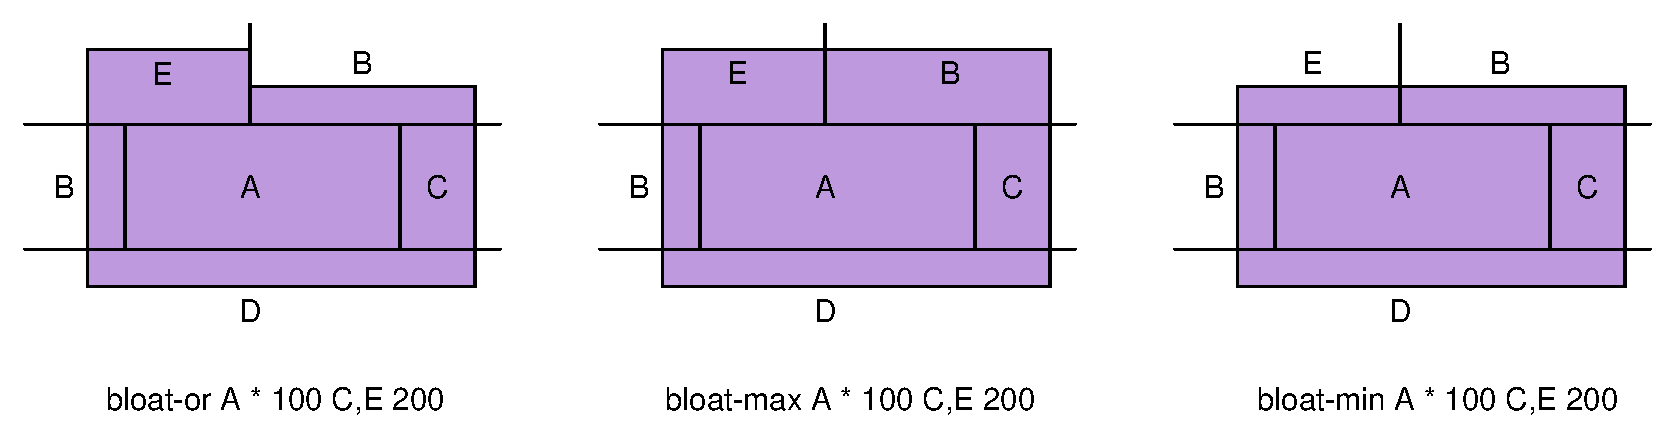
\epsfig{file=../psfigures/maint2.2.ps, width=\columnwidth}
      \caption{The three different forms of {\bfseries bloat} behave
	slightly differently when two different bloat distances apply
	along the same side of a tile.  In each of the above examples,
	the CIF that would be generated is shown in bold outline.
	If {\bfseries bloat-or} is specified, a jagged edge may
	be generated, as on the left.  If {\bfseries bloat-max} is used,
	the largest bloat distance for each side is applied uniformly to
	the side, as in the center.  If {\bfseries bloat-min} is used, the
	smallest bloat distance for each side is applied uniformly to the
	side, as on the right.}
   \end{center}
   \label{bloat}
\end{figure}

In retrospect, it's not clear that {\bfseries bloat-max} and {\bfseries bloat-min}
are very useful operations.  The problem is that they operate on tiles,
not regions.  This can cause unexpected behavior on concave regions.
For example, if the region being bloated is in the shape of a ``T'', a
single bloat factor will be applied to the underside of the horizontal
bar.  If you use {\bfseries bloat-max} or {\bfseries bloat-min}, you should
probably specify design-rules that require the shapes being bloated to
be convex.

The fourth bloat operation {\bfseries bloat-all} takes all tiles of
types {\itshape layers}, and grows to include all neighboring tiles of
types {\itshape layers2}.  This is very useful to generate marker layers
or implant layers for specific devices, where the marker or implant must
cover both the device and its contacts.  Take the material of the device
and use {\bfseries bloat-all} to expand into the contact areas.

An important geometric operation for creating contact cuts is
{\bfseries squares}.  It examines
each tile on the CIF plane, and replaces that tile with one or
more squares of material.  Each square is {\itshape size} CIF units
across, and squares are separated by {\itshape separation} units.  A border
of at least {\itshape border} units is left around the edge of the original
tile, if possible.  This operation is used to generate contact vias, as in
Figure~\ref{squares}.  If only one argument is given in the {\bfseries squares}
statement, then {\itshape separation} defaults to {\itshape size} and
{\itshape border} defaults to {\itshape size}/2.  If a tile doesn't hold an
integral number of squares, extra space is left around the edges of
the tile and the squares are centered in the tile.  If the tile is
so small that not even a single square can fit and still leave enough
border, then the border is reduced.  If a square won't fit in the
tile, even with no border, then no material is generated.
The {\bfseries squares} operation
must be used with some care, in conjunction with the design rules.
For example, if there are several adjacent skinny tiles, there
may not be enough room in any of the tiles for a square, so no
material will be generated at all.  Whenever you use the {\bfseries squares}
operator, you should use design rules to prohibit adjacent contact
tiles, and you should always use the {\bfseries no{\_}overlap} rule to prevent
unpleasant hierarchical interactions.  The problems with hierarchy
are discussed in Section~\ref{hierarchy} below, and design rules are discussed
in Section~\ref{s_mzrouter}.

\begin{figure}[ht]
   \begin{center}
      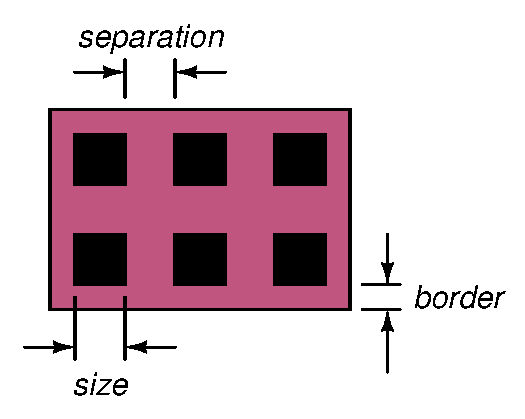
\epsfig{file=../psfigures/maint2.3.ps, width=0.33\columnwidth}
      \caption{The {\bfseries squares} operator chops each tile up
	into squares, as determined by the {\itshape border}, {\itshape size},
	and {\itshape separation} parameters.  In the example, the bold
	lines show the CIF that would be generated by a {\bfseries squares}
	operation.  The squares of material are always centered so that
	the borders on opposite sides are the same.}
      \label{squares}
   \end{center}
\end{figure}

The {\bfseries squares-grid} operator is similar to {\bfseries squares} and
takes the same arguments, except for the additional optional {\itshape x} and
{\itshape y} offsets (which default to 1).  Where the {\bfseries squares}
operator places contacts on the half-lambda grid, the {\bfseries squares-grid}
operator places contacts on an integer grid of {\itshape x} and {\itshape y}.
This is helpful where manufacturing grid limitations do not allow half-lambda
coordinates.  However, it is necessary then to enforce a ``no-overlap'' rule
for contacts in the DRC section to prevent incorrect contacts cuts from
being generated in overlapping subcells.  The {\bfseries squares-grid}
operator can also be used with {\itshape x} and {\itshape y} values to
generate fill geometry, or to generate offset contact cut arrays for pad
vias.

The {\bfseries slots} operator is similar to {\bfseries squares} operator,
but as the name implies, the resulting shapes generated are rectangular,
not (necessarily) square.  Slots are generated inside individual tiles,
like the squares operator, so each slots operation is separately oriented
relative to the tile's long and short edges.  Separate border, size, and
separation values can be specified for the short and long dimensions of
the tile.  This operator can be used in a number of situations:

\begin{enumerate}
   \item Generate square contact cuts with different border requirements on
	the short and long sides, as required for a number of deep submicron
	processes like 90 nanometer.
   \item Automatically generate slots in large metal areas, which most
	processes require.  Note, however, that it is impossible to
	correctly generate all slots, so this cannot completely replace
	the widespacing DRC rule.
   \item Generate slot contacts.
   \item Generate fill geometry.
   \item Generate marker layers for resitors that abut the position of
	contacts, a generally-accepted way to define a resistor area
	boundary.
\end{enumerate}

Note that the {\bfseries slots} operator comes in three different forms
with different numbers of arguments.  With only three arguments (short
side description only), the {\bfseries slots} operator creates stripes
that extend to the edge of the tile.  With four arguments (short side
description plus long side border dimension only), the {\bfseries slots}
operator create stripes that extend to the edge of the tile, with
an appropriate border spacing at each end.  In these two cases, the
slots have variable length that is set by the size of the tile.  In the
final form, all short and long side dimensions are declared.  The
generated slots are of fixed size, and like the {\bfseries squares}
operator, their positions will be adjusted to center them on the tile.
The {\itshape offset} is intended to let each row of slots be offset
from the previous one by a fixed amount, but is currently unimplemented
and has no effect.

\begin{figure}[ht]
   \begin{center}
      \epsfig{file=../psfigures/maint2.3b.ps, width=0.6\columnwidth}
      \caption{The {\bfseries slots} operator chops each tile up
	into rectangles.}
      \label{slots}
   \end{center}
\end{figure}

The {\bfseries bbox} operator generates a single rectangle that encompasses
the bounding box of the cell.  This is useful for the occasional process
that requires marker or implant layers covering an entire design.  The
variant {\bfseries bbox top} will generate a rectangle encompassing the
bounding box of the cell, but will only do so for the top-level cell of the
design.

\subsection{Labels}

There is an additional statement permitted in the {\bfseries cifoutput}
section as part of a layer description:

\starti
   \ii {\bfseries labels} {\itshape Magiclayers}
\endi

This statement tells Magic that labels attached to Magic layers
{\itshape Magiclayers} are to be associated with the current CIF layer.
Each Magic layer should only appear in one such statement for
any given CIF style.  If a Magic layer doesn't appear in any
{\bfseries labels} statement, then it is not attached to a specific
layer when output in CIF.

\subsection{Calma (GDS II Stream format) layers}

Each layer description in the {\bfseries cifoutput} section may also
contain one of the following statements:

\starti
   \ii {\bfseries gds} {\itshape gdsNumber} {\itshape gdsType} \\
   \ii {\bfseries calma} {\itshape gdsNumber} {\itshape gdsType}
\endi

Although the format is rarely referred to as ``Calma'' anymore, the
keyword is retained for backwards compatibility with format 27 (and
earlier) files.

This statement tells Magic which layer number and data type
to use when the {\bfseries gds} command outputs GDS II Stream format
for this defined CIF layer.
Both {\itshape gdsNumber} and {\itshape gdsType} should be positive
integers, between 0 and 63.
Each CIF layer should have a different {\itshape gdsNumber}.
If there is no {\bfseries gds} line for a given CIF layer, then
that layer will not be output by the ``{\bfseries gds write}'' command.
The reverse is not true:  every generated output layer must have a
defined CIF layer type, even if the foundry only supports GDS format.
In such case, the CIF layer name may violate the restrictive 4-character
format required by the CIF syntax specification, and may be used to
provide a reasonable, human-readable descriptive name of the GDS layer.

\begin{figure}[ht]
   \begin{center}
      \epsfig{file=../psfigures/maint2.4.ps, width=0.85\columnwidth}
      \caption{If the operator {\bfseries grow 100} is applied to the
	shapes in (a), the merged shape in (b) results.  If the operator
	{\bfseries shrink 100} is applied to (b), the result is (c).  However,
	if the two original shapes in (a) belong to different cells, and
	if CIF is generated separately in each cell, the result will be
	the same as in (a).  Magic handles this by outputting additional
	information in the parent of the subcells to fill in the gap between
	the shapes.}
      \label{growshrink}
   \end{center}
\end{figure}

\subsection{Hierarchy} \label{hierarchy}

Hierarchical designs make life especially difficult for the
CIF generator.  The CIF corresponding
to a collection of subcells may not necessarily be the same
as the sum of the CIF's of the individual cells.  For example,
if a layer is generated by growing and then shrinking, nearby
features from different cells may merge together so that they
don't shrink back to their original shapes (see Figure~\ref{growshrink}).
If Magic
generates CIF separately for each cell, the interactions between
cells will not be reflected properly.  The CIF generator attempts
to avoid these problems.  Although it generates CIF in a
hierarchical representation that matches the Magic cell structure,
it tries to ensure that the resulting CIF patterns are exactly the same
as if the entire Magic design had been flattened into a single cell
and then CIF were generated from the flattened design.  It does this
by looking in each cell for places where subcells are close enough
to interact with each other or with paint in the parent.  Where this
happens, Magic flattens the interaction area and generates CIF for
it;  then Magic flattens each of the subcells separately and generates
CIF for them.  Finally, it compares the CIF from the subcells with the
CIF from the flattened parent.  Where there is a difference, Magic
outputs extra CIF in the parent to compensate.

Magic's hierarchical approach only works if the overall CIF for the
parent ends up covering at least as much area as the CIFs for the
individual components, so all compensation can be done by adding
extra CIF to the parent.  In mathematical terms, this requires
each geometric operation to obey the rule

\starti
   \ii Op(A $\cup$ B) $\supseteq$ Op(A) $\cup$ Op(B)
\endi

The operations {\bfseries and}, {\bfseries or}, {\bfseries grow}, and
{\bfseries shrink} all
obey this rule.  Unfortunately, the {\bfseries and-not}, {\bfseries bloat},
and {\bfseries squares}
operations do not.  For example, if there are two partially-overlapping
tiles in different cells, the squares generated from one of the cells
may fall in the separations between squares in the other cell, resulting
in much larger areas of material than expected.
There are two ways around this problem.  One
way is to use the design rules to prohibit problem situations from
arising.  This applies mainly to the {\bfseries squares} operator.  Tiles
from which squares are made should never be allowed to overlap
other such tiles in different cells unless the overlap is exact,
so each cell will generate squares in the same place.  You can
use the {\bfseries exact{\_}overlap} design rule for this.

The second approach is to leave things up to the designer.
When generating CIF, Magic issues warnings where there is less material
in the children than the parent.  The designer can locate these problems
and eliminate the interactions that cause the trouble.  Warning:
Magic does not check the {\bfseries squares} operations for hierarchical
consistency, so you absolutely must use {\bfseries exact{\_}overlap} design
rule checks! Right now, the {\bfseries cifoutput} section of the
technology is one of the trickiest things in the whole file, particularly
since errors here may not show up until your chip comes back and doesn't
work.  Be extremely careful when writing this part!

\begin{table}[ht!]
   \begin{center}
      \begin{tabular}{|l|} \hline
	   {\bfseries cifinput} \\
	   style lambda=1.0(gen) \\
    	   \I scalefactor 100 \\
    	   \I layer m1 CMF \\
           \II  labels CMF \\
    	   \I layer ndiff CSN \\
           \II  and CAA \\
    	   \I layer nsd CWN \\
           \II  and CSN \\
           \II  and CAA \\
    	   \I layer nfet CPG \\
           \II  and CAA \\
           \II  and CSN \\
    	   \I layer ndc CCA \\
           \II  grow 100 \\
           \II  and CAA \\
           \II  and CWP \\
           \II  and CSN \\
           \II  and CMF \\
    	   \I layer nncont CCA \\
           \II  grow 100 \\
           \II  and CAA \\
           \II  and CSN \\
           \II  and CWN \\
           \II  and CMF \\
    	   \I calma CAA 1 * \\
    	   \I calma CCA 2 * \\
    	   \I calma CMF 4 * \\
    	   \I calma CPG 7 * \\
    	   \I calma CSN 8 * \\
    	   \I calma CWN 11 * \\
    	   \I calma CWP 12 * \\
	   {\bfseries end} \\ \hline
      \end{tabular}
      \caption{Part of the {\bfseries cifinput} section.  The order of
	the layers is important, since each Magic layer overrides the
	previous ones just as if they were painted by hand.}
      \label{cifinput}
   \end{center}
\end{table}

Another problem with hierarchical generation is that it can be very
slow, especially when there are a number of rules in the cifoutput
section with very large grow or shrink distances, such that magic
must always expand its area of interest by this amount to be sure
of capturing all possible layer interactions.  When this ``halo''
distance becomes larger than the average subcell, much of the
design may end up being processed multiple times.  Noticeably slow
output generation is usually indicative of this problem.  It can
be alleviated by keeping output rules simple.  Note that basic AND
and OR operations do not interact between subcells, so that rules
made from only these operators will not be processed during subcell
interaction generation.  Remember that typically, subcell interaction
paint will only be generated for layers that have a ``grow'' operation
followed by a ``shrink'' operation.  This common ruleset lets layers
that are too closely spaced to be merged together, thus eliminating
the need for a spacing rule between the layers.  But consider carefully
before implementing such a rule.  Implementing a DRC spacing rule
instead may eliminate a huge amount of output processing.  Usually
this situation crops up for auto-generated layers such as implants and
wells, to prevent magic from auto-generating DRC spacing violations.
But again, consider carefully whether it might be better to require
the layout engineer to draw the layers instead of attempting to
auto-generate them.

\subsection{Render statements}

At the end of each style in the {\bfseries cifoutput} section, one may
include {\bfseries render} statements, one per defined CIF/GDS layer.
These {\bfseries render} statements are used by the 3-D drawing window
in the OpenGL graphics version of magic, and are also used by the
``{\bfseries cif see}'' command to set the style painted.  The syntax
for the statement is as follows:

\starti
   \ii {\bfseries render} {\itshape cif\_layer style\_name height thickness}
\endi

The {\itshape cif\_layer} is any valid layer name defined in the same
{\bfseries cifoutput} section where the {\bfseries render} statement occurs.
The {\itshape style\_name} is the name or number of a style in the styles
file.  The names are the same as used in the {\bfseries styles} section of
the technology file.  {\itshape height} and {\itshape thickness} are
effectively dimensionless units and are used for relative placement and
scaling of the three-dimensional layout view (such views generally have
a greatly expanded z-axis scaling).  By default, all layers are given the
same style and a zero height and thickness, so effectively nothing useful
can be seen in the 3-D view without a complete set of {\bfseries render}
statements.

\section{Cifinput section}

In addition to writing CIF, Magic can also read in CIF files using
the {\bfseries :cif read} {\itshape file} command.  The {\bfseries cifinput}
section of the technology file describes how to convert from CIF mask layers
to Magic tile types.
In addition, it provides information to the Calma reader to allow
it to read in Calma GDS II Stream format files.
The {\bfseries cifinput} section is very similar to the {\bfseries cifoutput}
section.  It can contain several styles, with a line of the form

\starti
   \ii {\bfseries style} {\itshape name}
\endi

used to end the description of the previous style (if any), and start a
new CIF input style called {\itshape name}.  If no initial style name is
given, the name {\bfseries default} is assigned.  Each style must have a
statement of the form

\starti
   \ii {\bfseries scalefactor} {\itshape scale} {\bfseries [nanometers]}
\endi

to indicate the output scale relative to Magic units.  Without the
optional keyword {\bfseries nanometers}, {\itshape scale} describes how
many hundredths of a micron correspond to one unit in Magic.  With
{\bfseries nanometers} declared, {\itshape scale} describes how many
nanometers correspond to one unit in Magic.

Like the {\bfseries cifoutput} section, each style consists of a number
of layer descriptions.  A layer description contains one
or more lines describing a series of geometric operations to be
performed on CIF layers.  The result of all these operations is
painted on a particular Magic layer just as if the user had
painted that information by hand.
A layer description begins with a statement of the form

\starti
   \ii {\bfseries layer} {\itshape magicLayer }[{\itshape layers}]
\endi

In the {\bfseries layer} statement, {\itshape magicLayer} is the Magic layer
that will be painted after performing the geometric operations,
and {\itshape layers} is an optional list of CIF layers.  If
{\itshape layers} is specified, it is the initial value for the layer
being built up.  If {\itshape layers} isn't specified, the layer starts
off empty.  As in the {\bfseries cifoutput} section, each line after
the {\itshape layer} statement gives a geometric operation that is applied
to the previous contents of the layer being built in order to generate
new contents for the layer.  The result of the last geometric operation
is painted into the Magic database.

The geometric operations that are allowed in the {\bfseries cifinput} section
are a subset of those permitted in the {\bfseries cifoutput} section:

\starti
   \ii {\bfseries or} {\itshape layers} \\
   \ii {\bfseries and} {\itshape layers} \\
   \ii {\bfseries and-not} {\itshape layers} \\
   \ii {\bfseries grow} {\itshape amount} \\
   \ii {\bfseries shrink} {\itshape amount}
\endi

In these commands the {\itshape layers} must all be CIF layers, and the
{\itshape amounts} are all CIF distances (centimicrons, unless the keyword
{\bfseries nanometers} has been used in the {\bfseries scalefactor}
specification).  As with the
{\bfseries cifoutput} section, layers can only be specified in simple
comma-separated lists:  tildes and slashes are not permitted.

When CIF files are read, all the mask information is read for a cell
before performing any of the geometric processing.  After the cell
has been completely read in, the Magic layers are produced and
painted in the order they appear in the technology file.  In
general, the order that the layers are processed is important
since each layer will usually override the previous ones.  For
example, in the scmos tech file shown in Table~\ref{cifinput} the commands
for {\bfseries ndiff} will result in the {\bfseries ndiff} layer being generated
not only where there is only ndiffusion
but also where there are
ntransistors and ndcontacts.
The descriptions
for {\bfseries ntransistor} and {\bfseries ndcontact} appear later in the section,
so those layers will replace the {\bfseries ndiff} material that was originally
painted.

Labels are handled in the {\bfseries cifinput} section just like in the
{\bfseries cifoutput} section.  A line of the form

\starti
   \ii {\bfseries labels} {\itshape layers}
\endi

means that the current Magic layer is to receive all CIF labels
on {\itshape layers}.  This is actually just an initial layer assignment
for the labels.  Once a CIF cell has been read in, Magic scans the
label list and re-assigns labels if necessary.  In the example of
Table~\ref{cifinput}, if a label is attached to the CIF layer CPG then it will
be assigned to the Magic layer {\bfseries poly}.  However, the polysilicon
may actually be part of a poly-metal contact, which is Magic layer
{\bfseries pcontact}.  After all the mask information has been processed, 
Magic checks the material underneath the layer, and adjusts the
label's layer to match that material ({\bfseries pcontact} in this case).
This is the same as what would happen if a designer painted {\bfseries poly}
over an area, attached a label to the material, then painted {\bfseries pcontact}
over the area.

No hierarchical mask processing is done for CIF input.  Each cell
is read in and its layers are processed independently
from all other cells;  Magic assumes that there
will not be any unpleasant interactions between cells as happens
in CIF output (and so far, at least, this seems to be a valid
assumption).

If Magic encounters a CIF layer name that doesn't appear
in any of the lines for the current CIF input style, it
issues a warning message and ignores the information associated
with the layer.  If you would like Magic to ignore certain
layers without issuing any warning messages, insert a line
of the form

\starti
   \ii {\bfseries ignore} {\itshape cifLayers}
\endi

where {\itshape cifLayers} is a comma-separated list of one or
more CIF layer names.

Calma layers are specified via {\bfseries calma} lines, which should appear
at the end of the {\bfseries cifinput} section.  They are of the form:

\starti
   \ii {\bfseries calma} {\itshape cifLayer} {\itshape calmaLayers}
	{\itshape calmaTypes}
\endi

The {\itshape cifLayer} is one of the CIF types mentioned in the {\bfseries cifinput}
section.  Both {\itshape calmaLayers} and {\itshape calmaTypes} are one or more
comma-separated integers between 0 and 63.  The interpretation of
a {\bfseries calma} line is that any Calma geometry whose layer is any
of the layers in {\itshape calmaLayers}, and whose type is any of the
types in {\itshape calmaTypes}, should be treated as the CIF layer
{\itshape cifLayer}.
Either or both of {\itshape calmaLayers} and {\itshape calmaTypes} may be
the character {\bfseries *} instead of a comma-separated list of integers;
this character means {\itshape all} layers or types respectively.
It is commonly used for {\itshape calmaTypes} to indicate that the
Calma type of a piece of geometry should be ignored.

Just as for CIF, Magic also issues warnings if it encounters
unknown Calma layers while reading Stream files.  If there are
layers that you'd like Magic to ignore without issuing warnings,
assign them to a dummy CIF layer and ignore the CIF layer.

\section{Lef section}

This section defines a mapping between magic layers and layers that may
be found in LEF and DEF format files.  Without the section, magic cannot
read a LEF or DEF file.  The LEF and DEF layer declarations are usually
simple and straightforward (as they typically define metal layers only),
so often it will suffice to insert a plain vanilla {\bfseries lef} section
into a technology file if one is missing.  The {\bfseries lef} section
was introduced in technology file format 28, and is therefore absent from
all {\ttfamily .tech27} technology files.   All of the statements in
the {\bfseries lef} section have the same format:

\starti
   \ii {\bfseries layer} {\itshape magic-type lefdef-type} \dots \\
   \ii {\bfseries cut} {\itshape magic-type lefdef-type} \dots \\
   \ii {\bfseries route}\vbar {\bfseries routing} {\itshape magic-type lefdef-type}
	\dots \\
   \ii {\bfseries obstruction} {\itshape magic-type lefdef-type} \dots \\
   \ii {\bfseries masterslice} {\itshape magic-type lefdef-type} \dots \\
   \ii {\bfseries overlap} {\itshape magic-type lefdef-type} \dots
\endi

Each statement defines a mapping between a Magic layer type
{\itshape magic-type} and one or more type names {\itshape lefdef-type} 
(space-separated) that might be encountered in a LEF or DEF file.  The
different command names all refer to different type classes defined
by the LEF/DEF specification.  For most purposes, it is only necessary
to use the {\bfseries layer} statement.  If the magic type is a contact
type, then the {\bfseries layer} statement is equivalent to specifying
{\bfseries cut};  otherwise, it is equivalent to {\bfseries route}.

Table \ref{lefdef} is a typical {\bfseries lef} section for a 5-metal technology,
which encompasses the most commonly used layer names found in LEF and DEF files.

\begin{table}[ht]
   \begin{center}
      \begin{tabular}{|lllllll|} \hline
	  {\bfseries lef} &&&&&& \\
	  & masterslice & ndiff & diffusion & active && \\
	  & masterslice & poly & poly & POLY1 & pl & \\
	  & routing & m1 & m1 & metal1 & METAL1 & METAL\_1 \\
	  & routing & m2 & m2 & metal2 & METAL2 & METAL\_2 \\
	  & routing & m3 & m3 & metal3 & METAL3 & METAL\_3 \\
	  & routing & m4 & m4 & metal4 & METAL4 & METAL\_4 \\
	  & routing & m5 & m5 & metal5 & METAL5 & METAL\_5 \\
	  &&&&&&\\
	  & cut & pc & cont1 & pl-m1 && \\
	  & cut & m2c & via1 & cont2 & VIA12 & m1-m2 \\
	  & cut & m3c & via2 & cont3 & VIA23 & m2-m3 \\
	  & cut & m4c & via3 & cont4 & VIA34 & m3-m4 \\
	  & cut & m5c & via4 & cont5 & VIA45 & m4-m5 \\
	  &&&&&& \\
	  & overlap & comment & overlap & OVERLAP && \\
	  {\bfseries end} &&&&&& \\ \hline
      \end{tabular}
      \caption{A plain vanilla lef section.}
      \label{lefdef}
   \end{center}
\end{table}

\section{Mzrouter section} \label{s_mzrouter}

This section defines the layers and contacts available to the Magic maze router, {\itshape mzrouter}, and assigns default costs for each type.  Default widths 
and spacings are
derived from the {\bfseries drc} section of the technology file (described below) 
but can be overridden in this 
section.  Other mzrouter parameters, for example, search rate and width, 
can also be specified in this section.  The syntax and function of the
lines in the {\bfseries mzrouter} section of the technology file 
are specified in the subsections below.  Each
set of specifications should be headed by a {\bfseries style} line.
{\bfseries Routelayer}
and {\bfseries routecontact} specifications should precede references to them.

\begin{table}[ht]
   \begin{center}
      \begin{tabular}{|llllll|} \hline
	  {\bfseries mzrouter} &&&&& \\
	  style & irouter &&&& \\
	  layer		& m2		& 32	& 64	& 256	& 1 \\
	  layer		& m1		& 64	& 32	& 256	& 1 \\
	  layer		& poly		& 128	& 128	& 512	& 1 \\
	  contact	& m2contact	& metal1 & metal2 & 1024 & \\
	  contact	& pcontact	& metal1 & poly	& 2056 & \\
	  notactive	& poly		& pcontact &&& \\
	  style & garouter &&&& \\
	  layer		& m2	& 32	& 64	& 256	& 1 \\
	  layer		& m1	& 64	& 32	& 256	& 1 \\
	  contact	& m2contact	& metal1 & metal2 & 1024 & \\
	  {\bfseries end} &&&&& \\ \hline
      \end{tabular}
      \caption{Mzrouter section for the scmos technology.}
      \label{mzrouter}
   \end{center}
\end{table}

\subsection{Styles}

The mzrouter is currently used in two contexts, 
interactively via the {\bfseries iroute} command, and as a subroutine to the garouter
for stem generation.  To permit distinct parameters for these two
uses, the lines in the {\bfseries mzrouter} section are grouped into {\itshape styles}.
The lines pertaining to the irouter should be preceded by 

\starti
   \ii {\bfseries style irouter}
\endi

and those pertaining to the garouter should be preceded by the specification

\starti
   \ii {\bfseries style garouter}
\endi

Other styles can be specified, but are currently not used.
Table~\ref{mzrouter} shows the mzrouter section from the scmos technology.

\subsection{Layers}

Layer lines
define the route-layers available to the maze router in that style.  They
have the following form:

\starti
   \ii {\bfseries layer} {\itshape type hCost vCost jogCost hintCost}
\endi

Here {\itshape type} is the name of the tiletype of the layer and {\itshape hCost},
{\itshape vCost}, {\itshape jogCost} and {\itshape hintCost}, are non-negative integers
specifying the cost per unit horizontal distance, 
cost per unit vertical distance, cost per jog, and 
cost per unit area of deviation from magnets, respectively.  Route layers
for any given style must lie in distinct planes.

\subsection{Contacts}

Contact lines specify
the route-contacts available to the mzrouter in the current
style.   They have the following form:

\starti
   \ii {\bfseries contact} {\itshape type routeLayer1 routeLayer2 cost}
\endi

Here {\itshape type} is the tiletype of the contact, {\itshape routeLayer1} and
{\itshape routeLayer2} are the two layers connected by the contact, and {\itshape cost}
is a nonnegative integer specifying the cost per contact.

\subsection{Notactive}

It maybe desirable to have a layer or contact available to the maze router, 
but default to off, i.e., not be used by the mzrouter until explicitly
made active.  Route-types (route-layers or route-contacts) can be made to 
default to off with the following specification:

\starti
   \ii {\bfseries notactive} {\itshape route-type} \dots [{\bfseries route-typen}]
\endi

\subsection{Search}

The search {\bfseries rate}, {\bfseries width}, and {\bfseries penalty} parameters can 
be set with a specification of the form:

\starti
   \ii {\bfseries search} {\itshape  rate width penalty}
\endi

Here {\itshape rate} and {\itshape width} are positive integers.  And {\itshape penalty}
is a positive rational (it may include a decimal point).  See the irouter
tutorial for a discussion of these parameters.  (Note that {\bfseries penalty}
is a ``wizardly'' parameter, i.e., it is interactively
set and examined via {\bfseries iroute wizard} not {\bfseries iroute search}).
If no {\bfseries search} line
is given for a style, the overall mzrouter defaults are used.

\subsection{Width}

Appropriate widths for route-types are normally derived from the {\bfseries drc}
section
of the technology file.  These can be overridden with width specifications
of the following form:

\starti
   \ii {\bfseries width} {\itshape route-type width}
\endi

Here {\itshape width} is a positive integer.

\subsection{Spacing}

Minimum spacings between routing on a route-type and other types are
derived from the design rules.  These values can be overridden by explicit
spacing specifications in the {\bfseries mzrouter} section.  Spacing 
specifications have the following form:

\starti
   \ii {\bfseries spacing} {\itshape  routetype type1 spacing1 } \dots
	 [{\itshape typen spacingn}]
\endi

Spacing values must be nonnegative integers or {\bfseries NIL}.  The special type
{\bfseries SUBCELL} can be used to specify minimum spacing to unexpanded subcells.

\section{Drc section}

The design rules used by Magic's design rule checker
come entirely from the technology file.
We'll look first at two simple kinds of rules,
{\bfseries width} and and {\bfseries spacing}.
Most of the rules in the {\bfseries drc}
section are one or the other of these kinds of rules.

\subsection{Width rules}

The minimum width of a collection of types, taken together,
is expressed by a {\bfseries width} rule.
Such a rule has the form:

\starti
   \ii {\bfseries width} {\itshape type-list width error}
\endi

where {\itshape type-list} is a set of tile types
(see Section~\ref{typelists} for syntax),
{\itshape width} is an integer, and {\itshape error}
is a string, enclosed in double quotes,
that can be printed by the command {\bfseries :drc why}
if the rule is violated.
A width rule requires that all regions containing any types
in the set {\itshape types} must be wider than {\itshape w} in both dimensions.
For example, in Table~\ref{drcwidth}, the rule

\starti
   \ii {\bfseries width} nwell 6 {\itshape {\q}N-Well width must be at least 6
	(MOSIS rule \#1.1){\q}}
\endi

means that nwells must be at least 6 units
wide whenever they appear.
The {\itshape type-list}
field may contain more than a single type, as in the following rule:

\starti
   \ii {\bfseries width} allDiff 2 {\itshape {\q}Diffusion width must
	be at least 2 (MOSIS rule \#2.1){\q}}
\endi

which means that all regions consisting of the types
containing any kind of diffusion
be at least 2 units wide.
Because many of the rules in the {\bfseries drc} section refer to the
same sets of layers, the {\bfseries \#define} facility of the C preprocessor
is used to define a number of macros for these sets of layers.
Table~\ref{drctiles} gives a complete list.

\begin{table}[ht]
   \begin{center}
      \begin{tabular}{|lll|} \hline
	\#define & allDiff & ndiff,pdiff,ndc/a,pdc/a,ppcont/a,nncont/a,pfet,nfet,psd,nsd
		\\
	\#define & extPoly & poly,pcontact \\
	\#define & extM1   & metal1,pcontact/m1,ndc/m1,ppcont/m1,pdc/m1,nncont/m1 \\
	\#define & extM2   & metal2,m2contact/m2 \\ \hline
      \end{tabular}
      \caption{Abbreviations for sets of tile types.}
      \label{drctiles}
   \end{center}
\end{table}

\begin{table}[ht]
   \begin{center}
      \begin{tabular}{|llll|} \hline
	width &	pwell	& 6 & {\q}P-Well width must be at least 6
		(MOSIS rule \#1.1){\q} \\
	width &	nwell	& 6 & {\q}N-Well width must be at least 6
		(MOSIS rule \#1.1){\q} \\
	width &	allDiff	& 2 & {\q}Diffusion width must be at least 2
		(MOSIS rule \#2.1){\q} \\
	width &	allPoly	& 2 & {\q}Polysilicon width must be at least 2
		(MOSIS rule \#3.1){\q} \\ \hline
      \end{tabular}
      \caption{Some width rules in the {\bfseries drc} section.}
      \label{drcwidth}
   \end{center}
\end{table}

All of the layers named in any one width rule must lie on the
same plane.  However, if some of the layers are contacts, Magic
will substitute a different contact image if the named image
isn't on the same plane as the other layers.

\subsection{Spacing rules}

The second simple kind of design rule is a {\bfseries spacing} rule.
It comes in two flavors:
{\bfseries touching{\_}ok}, and {\bfseries touching{\_}illegal},
both with the following syntax:

\starti
   \ii {\bfseries spacing} {\itshape types1 types2 distance flavor error}
\endi

The first flavor, {\bfseries touching{\_}ok}, does not prohibit
{\itshape types1} and {\itshape types2} from being immediately adjacent.
It merely requires that any type in the set {\itshape types1}
must be separated by a ``Manhattan'' distance of at least
{\itshape distance} units from any type in the set {\itshape types2}
that is not immediately adjacent to the first type.
See Figure~\ref{distance} for an illustration of Manhattan distance
for design rules.
As an example, consider the metal1 separation rule:

\starti
   \ii {\bfseries spacing} allPoly allPoly 2 {\bfseries touching{\_}ok} {\bk} \\
   \ii\> {\itshape {\q}Polysilicon spacing must be at least 2 (MOSIS rule \#3.2){\q}}
\endi

\begin{figure}[ht]
   \begin{center}
      \epsfig{file=../psfigures/maint2.5.ps, width=0.4\columnwidth}
      \caption{For design rule checking, the Manhattan distance between
	two horizontally or vertically aligned points is just the normal
	Euclidean distance.  If they are not so aligned, then the Manhattan
	distance is the length of the longest side of the right triangle
	forming the diagonal line between the points.}
   \end{center}
   \label{distance}
\end{figure}

This rule is symmetric ({\itshape types1} is equal to {\itshape types2}),
and requires, for example, that a pcontact
be separated by at least 2 units from a piece of polysilicon.
However, this rule does not prevent the pcontact
from touching a piece of poly.  In {\bfseries touching{\_}ok} rules,
all of the layers in both {\itshape types1} and {\itshape types2} must be stored
on the same plane (Magic will substitute different contact
images if necessary).  

\begin{table}[ht]
   \begin{center}
      \begin{tabular}{|lllll|} \hline
	spacing	 & allPoly & allPoly & 2 & touching{\_}ok {\bk} \\
		 & \multicolumn{4}{l|}{{\itshape {\q}Polysilicon spacing must be
		   at least 2 (MOSIS rule \#3.2){\q}}} \\
	spacing	 & pfet	 & nncont,nnd &	3 & touching{\_}illegal {\bk} \\
		 & \multicolumn{4}{l|}{{\itshape {\q}Transistors must be separated
		   from substrate contacts by 3 (MOSIS rule \#4.1){\q}}} \\
	spacing	 & pc	 & allDiff    &	1 & touching{\_}illegal {\bk} \\
		 & \multicolumn{4}{l|}{{\itshape {\q}Poly contact must be 1 unit
		   from diffusion (MOSIS rule \#5B.6){\q}}} \\ \hline
      \end{tabular}
      \caption{Some spacing rules in the {\bfseries drc} section.}
      \label{drcspacing}
   \end{center}
\end{table}

{\bfseries TOUCHING{\_}OK SPACING} RULES DO NOT WORK
FOR VERY LARGE SPACINGS (RELATIVE TO THE TYPES INVOLVED).  SEE FIGURE 6
FOR AN EXPLANATION.  If the spacing to be checked is greater
than the width of one of the types involved plus either its self-spacing or 
spacing to a second involved type,
{\bfseries touching{\_}ok spacing} may not work properly:  a violation can
be masked by an intervening touching type.  In such cases the rule
should be written using the {\bfseries edge4way} construct described below. 

\begin{figure}[ht]
   \begin{center}
      \epsfig{file=../psfigures/maint2.6.ps, width=0.5\columnwidth}
      \caption{The {\bfseries touching{\_}ok} rules cancels spacing checks
	if the material is touching.  This means that even distant material
	won't be checked for spacing.  If the rule applied at edge A is a
	touching{\_}ok rule between material t1 and t2, then no check will
	be made between the t1 material and the t2 material on the far right
	side of the diagram.  If this check was desired, it could be
	accomplished in this case by a {\bfseries edge4way} check from edge
	B.  This would not work in general, though, because that check 
	could also be masked by material of type t2, causing the touching{\_}ok
	rule to be invoked.}
      \label{touchingok}
   \end{center}
\end{figure}

The second flavor of spacing rule, {\bfseries touching{\_}illegal}, disallows
adjacency.  It is used for rules where {\itshape types1} and {\itshape types2}
can never touch, as in the following:

\starti
   \ii {\bfseries spacing} pc allDiff 1 {\bfseries touching{\_}illegal} {\bk} \\
   \ii\> {\itshape {\q}Poly contact must be 1 unit from diffusion
		(MOSIS rule \#5B.6){\q}}
\endi

Pcontacts and any type of diffusion must be at least 1 unit apart;
they cannot touch.
In {\bfseries touching{\_}illegal}
rules {\itshape types1} and {\itshape types2} may not have any types in common:
it would be rather strange not to permit a type to touch itself.  In
{\bfseries touching{\_}illegal} rules, {\itshape types1}
and {\itshape types2} may be spread across multiple planes;  Magic will find
violations between material on different planes.

\subsection{Wide material spacing rules}

Many fabrications processes require a larger distance between layers when
the width and length of one of those layers exceeds a certain minimum
dimension.  For instance, a process might declare that the normal spacing
between metal1 lines is 3 microns.  However, if a metal1 line exceeds
a width of 100 microns, then the spacing to other unrelated metal1 lines
must increase to 10 microns.  This situation is covered by the
{\bfseries widespacing} rule.  The syntax for {\bfseries widespacing} is as
follows:

\starti
   \ii {\bfseries widespacing} {\itshape types1 wwidth types2 distance flavor error}
\endi

The {\bfseries widespacing} rule matches the syntax of {\bfseries spacing} in all
respects except for the addition of the parameter {\itshape wwidth}, which declares
the minimum width of layers of type(s) {\itshape types1} that triggers the rule.
So for the example above, the correct {\bfseries widespacing} rule would be
(assuming 1 magic unit = 1 micron):

\starti
   \ii {\bfseries widespacing} allMetal1 100 allMetal1 10 {\bfseries touching{\_}ok} {\bk} \\
   \ii\> {\itshape {\q}Space to wide Metal1 (length and width \grt 100) must be at least 10{\q}}
\endi

\begin{figure}[ht]
   \begin{center}
      \epsfig{file=../psfigures/maint2.6b.ps, width=0.8\columnwidth}
      \caption{The {\bfseries widespacing} rule covers situations like that
	shown above, in which material of type {\itshape t1} normally must
	be {\itshape dist} units away from type {\itshape t2} (situation A).
	However, if both dimensions of material type {\itshape t1} are
	larger than or equal to some width {\itshape wwidth} (situation B),
	then the spacing must be increased to {\itshape wdist}.}
      \label{widespacing}
   \end{center}
\end{figure}

\subsection{Surround rule}

The {\bfseries surround} rule specifies what distance a layer must surround
another, and whether the presence of the surrounding material is optional or
mandatory.  This rule is designed for materials which must {\itshape completely}
surround another, such as metal around a contact cut or MiM capacitor layer.
The syntax is:

\starti
   \ii {\bfseries surround} {\itshape types1 types2 distance presence error}
\endi

and states that the layers in {\itshape types2} must surround the layers
in {\itshape types1} by an amound {\itshape distance} lambda units.  The
value of {\itshape presence} must be one of the keywords {\bfseries
absence\_ok} or {\bfseries absence\_illegal}.  When {\itshape presence} is
{\bfseries absence\_illegal}, then types {\itshape types2} must always be
present when types {\itshape types1} are present. When {\itshape presence}
is {\bfseries absence\_ok}, types {\itshape types1} may exist outside of
types {\itshape types2} without error, but where they coincide, types
{\itshape types2} must overlap {\itshape types1} by the amount
{\itshape distance}. 

\subsection{Overhang rule} rule specifies what distance a layer must overhang
another at an intersection.  This is used, for example, to specify the length
of polysilicon end-caps on transistors, which is the distance that the
polysilicon gate must extend beyond the defined gate area of the transistor
to ensure a correctly operating device.  The syntax is:

\starti
   \ii {\bfseries overhang} {\itshape types1 types2 distance error}
\endi

and states that layers in {\itshape types1} must overhang layers in
{\itshape types2} by an amount {\itshape distance} lambda units.  The
rule flags the complete absence of types {\itshape types1}, but does not
prohibit the use of {\itshape types1} as a bridge (that is, with
types {\itshape types2} on either side of {\itshape types1}, which
will generally be covered by a separate spacing rule, and which may
have a different spacing requirement). 

\subsection{Rectangle-only rule}

The {\bfseries rect\_only} rule is used to denote layers that must be
rectangular;  that is, they cannot bend, or have notches or tabs.
Generally, this is used for contacts, so that the CIF output operator
{\bfseries squares} will be guaranteed to generate a correct contact.
This is due to magic's corner-stitching tile database, where bends,
notches, tabs, and slots will break up an otherwise continuous patch
of material into potentially many small tiles, each one of which
might be too small to fit a contact cut.

\starti
   \ii {\bfseries rect\_only} {\itshape types error}
\endi

\subsection{Edge rules}

The width and spacing rules just described are actually translated
by Magic into an underlying, edge-based rule format.  This underlying
format can handle rules more general than simple widths and spacings,
and is accessible to the writer of a technology file via {\bfseries edge} rules.
These rules are applied at boundaries between material of
two different types, in any of four directions as shown in Figure~\ref{tileedge}.
The design rule table contains a separate list of rules for each possible
combination of materials on the two sides of an edge.

\begin{figure}[ht]
   \begin{center}
      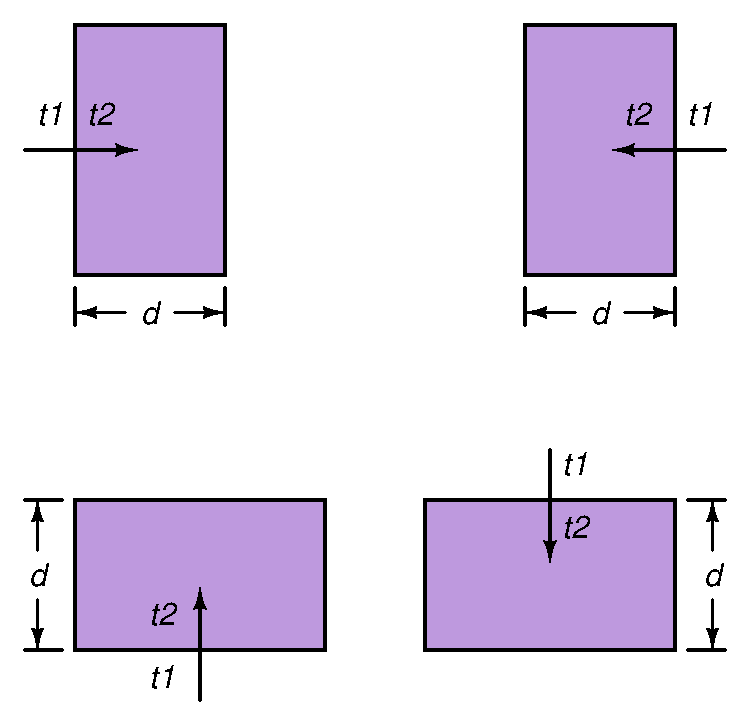
\epsfig{file=../psfigures/maint2.7.ps, width=0.4\columnwidth}
      \caption{Design rules are applied at the edges between tiles in
	the same plane.  A rule is specified in terms of type {\itshape t1}
	and type {\itshape t2}, the materials on either side of the edge.
	Each rule may be applied in any of four directions, as shown by
	the arrows.  The simplest rules require that only certain mask types
	can appear within distance {\itshape d} on {\itshape t2}'s side of
	the edge.}
      \label{tileedge}
   \end{center}
\end{figure}

In its simplest form, a rule specifies a distance
and a set of mask types:  only the given types are permitted
within that distance on {\itshape type2}'s side of the edge.
This area is referred to as the {\itshape constraint region}.
Unfortunately, this simple scheme will miss errors
in corner regions, such as the case shown in Figure~\ref{cornererror}.
To eliminate these problems, the full rule format allows the constraint
region to be extended past the ends of the edge under some
circumstances.
See Figure~\ref{cornerextend} for an illustration of the
corner rules and how they work.
Table~\ref{edgerules1} gives a complete
description of the information in each design rule.

\begin{figure}[hb!]
   \begin{center}
      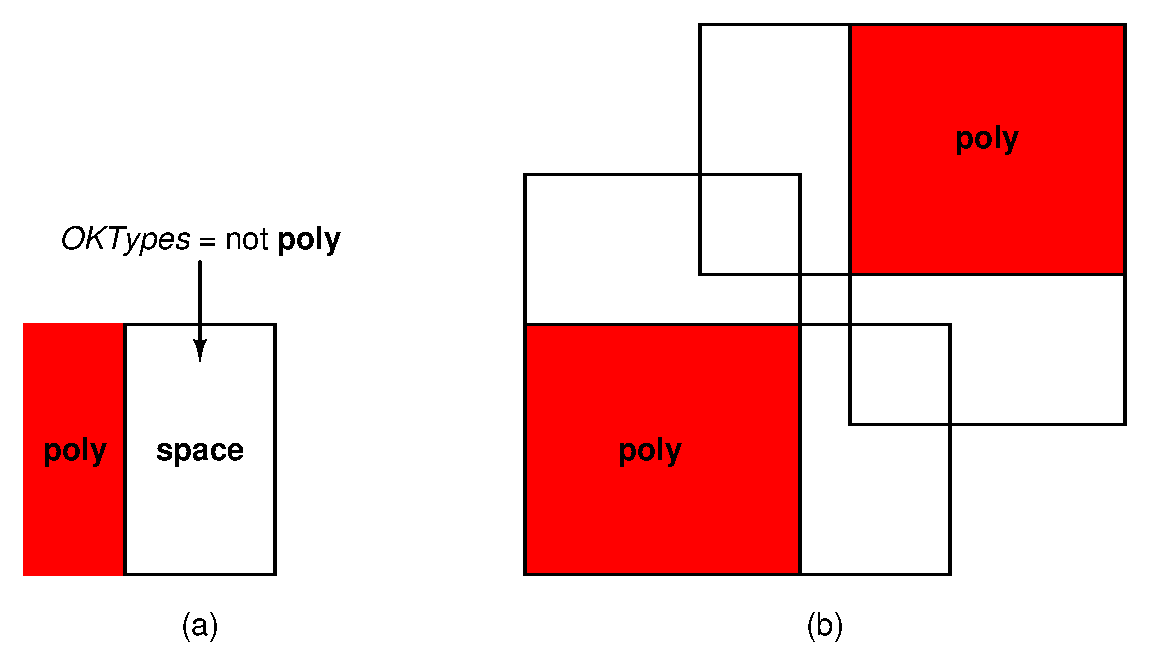
\epsfig{file=../psfigures/maint2.8.ps, width=0.7\columnwidth}
      \caption{If only the simple rules from Figure~\ref{tileedge} are used, errors
	may go unnoticed in corner regions.  For example, the polysilicon
	spacing rule in (a) will fail to detect the error in (b).}
      \label{cornererror}
   \end{center}
\end{figure}

\begin{figure}[ht!]
   \begin{center}
      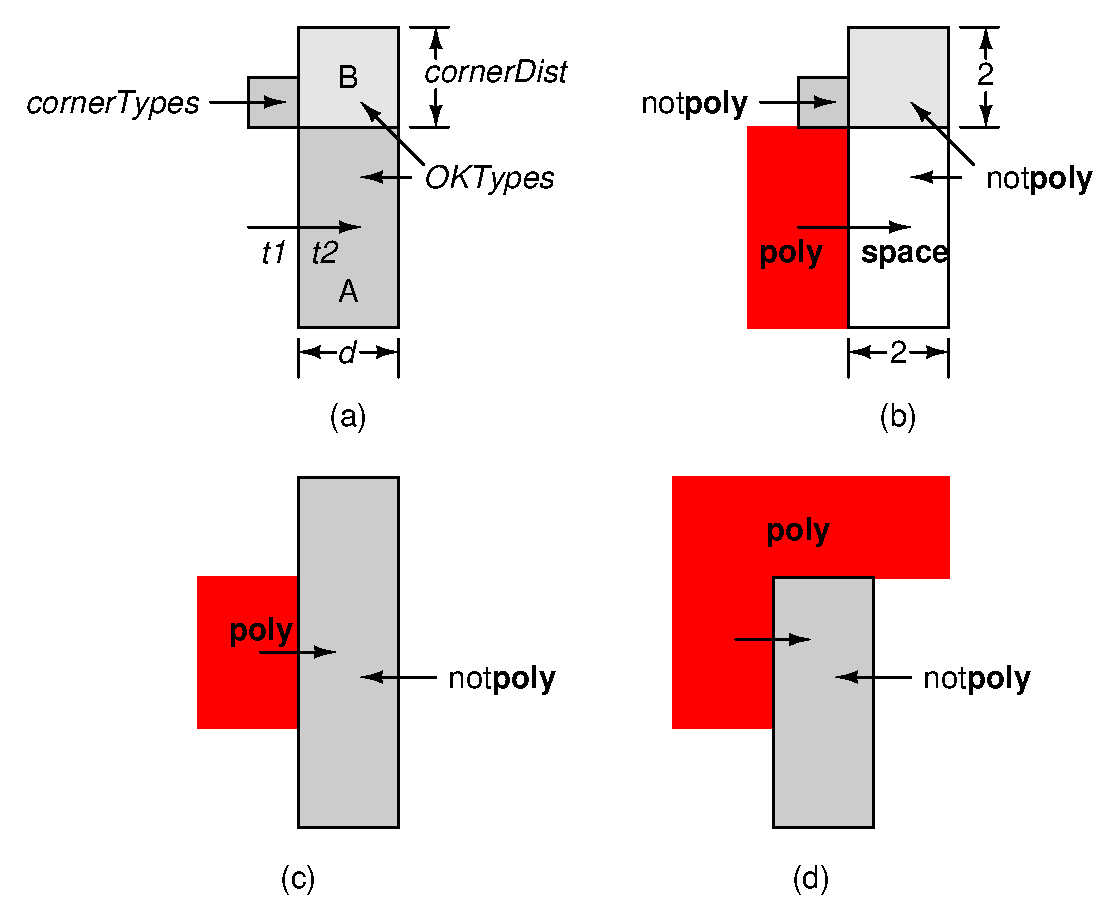
\epsfig{file=../psfigures/maint2.9.ps, width=0.75\columnwidth}
      \caption{The complete design rule format is illustrated in (a).
	Whenever an edge has {\itshape type1} on its left side and
	{\itshape type2} on its right side, the area A is checked to be
	sure that only {\itshape OKTypes} are present.  If the material
	just above and to the left of the edge is one of
	{\itshape cornerTypes}, then area B is also checked to be
	sure that it contains only {\itshape OKTypes}.  A similar
	corner check is made at the bottom of the edge.  Figure (b)
	shows a polysilicon spacing rule, (c) shows a situation where
	corner extension is performed on both ends of the edge, and
	(d) shows a situation where corner extension is made only at
	the bottom of the edge.  If the rule described in (d) were to
	be written as an {\bfseries edge} rule, it would look like:}
      \starti
	 \ii {\bfseries edge} poly space 2 \~{}poly \~{}poly 2 {\bk} \\
      	 \ii\> {\itshape {\q}Poly-poly separation must be at least 2{\q}}
      \endi
      \label{cornerextend}
   \end{center}
\end{figure}

\begin{table}[ht]
   \begin{center}
      \begin{tabular}{|l|p{0.5\columnwidth}|} \hline
	 Parameter   & 	Meaning \\ \hline \hline
	 type1	     &	Material on first side of edge. \\ \hline
	 type2	     &	Material on second side of edge. \\ \hline
	 d           &	Distance to check on second side of edge. \\ \hline
	 OKTypes     &	List of layers that are permitted within
			{\itshape d} units on second side of edge.
			({\itshape OKTypes}={\bfseries 0} means never OK) \\ \hline
	 cornerTypes &	List of layers that cause corner extension.  
			({\itshape cornerTypes}={\bfseries 0} means no
			corner extension) \\ \hline
	 cornerDist  &	Amount to extend constraint area when
			{\itshape cornerTypes} matches. \\ \hline
	plane	     &	Plane on which to check constraint region (defaults
			to same plane as {\itshape type1} and {\itshape type2}
			and {\itshape cornerTypes}). \\ \hline
      \end{tabular}
      \caption{The parts of an edge-based rule.}
      \label{edgerules1}
   \end{center}
\end{table}

Edge rules are specified in the technology file using the following syntax:

\starti
   \ii {\bfseries edge} {\itshape types1 types2 d OKTypes cornerTypes
	cornerDist error} [{\itshape plane}]
\endi

Both {\itshape types1} and {\itshape types2} are type-lists.
An edge rule is generated for each pair consisting of a type from
{\itshape types1} and a type from {\itshape types2}.  All the types in
{\itshape types1}, {\itshape types2}, and {\itshape cornerTypes} must lie
on a single plane.  See Figure~\ref{cornerextend} for an example edge rule.
It is sometimes
useful to specify a null list, i.e.,  {\bfseries 0}, for {\itshape OKTypes}
or {\itshape CornerTypes}.  Null {\itshape OKTypes} means no edges between
{\itshape types1} and {\itshape types2} are OK.  Null {\itshape CornerTypes}
means no corner extensions are to be checked (corner extensions are explained
below).

Some of the edge rules in Magic have the property that if a rule
is violated between two pieces of geometry, the violation can be
discovered looking from either piece of geometry toward the other.
To capitalize on this, Magic normally applies an edge
rule only in two of the four possible directions: bottom-to-top
and left-to-right, reducing the work it has to do by a factor of two.
Also, the corner extension is only performed to one side of the edge:
to the top for a left-to-right rule, and to the left for a bottom-to-top
rule.  All of the width and spacing rules translate neatly into edge
rules.

However, you'll probably find it easiest when you're writing
edge rules to insist that they be checked in all directions.
To do this, write the rule the same way except use the keyword
{\bfseries edge4way} instead of {\bfseries edge}:

\starti
   \ii {\bfseries edge4way} nfet ndiff 2 ndiff,ndc ndiff 2 {\bk} \\
   \ii\> {\itshape {\q}Diffusion must overhang transistor by at least 2{\q}}
\endi

Not only are {\bfseries edge4way} rules checked in all four directions,
but the corner extension is performed on {\itshape both} sides of the
edge.  For example, when checking a rule from left-to-right,
the corner extension is performed both to the top and to the bottom.
{\bfseries Edge4way} rules take twice as much time to check as {\bfseries edge}
rules, so it's to your advantage to use {\bfseries edge} rules wherever
you can.

\begin{table}[ht]
   \begin{center}
      \begin{tabular}{|lllllll|} \hline
	   edge4way &	ppcont,ppd &	ndiff,ndc,nfet & 3 & ndiff,ndc,nfet &
			ndiff,ndc,nfet &  3 {\bk} \\
	   & \multicolumn{5}{l}{{\itshape {\q}Ndiff must be 3 wide if it abuts
			ppcont or ppd (MOSIS rule \#??){\q}}} & \\
	   edge4way &	allPoly	 & \~{}(allPoly)/active & 3 & \~{}pc/active &
			\~{}(allPoly)/active &	3 {\bk} \\
	   & \multicolumn{5}{l}{{\itshape {\q}Poly contact must be at least 3 from
			other poly (MOSIS rule \#5B.4,5){\q}}} & \\
	   edge4way &	allPoly	 & \~{}(allPoly)/active	& 1 & \~{}m2c/metal2 &
			\~{}(allPoly)/active &	1 {\bk} \\
	   & \multicolumn{5}{l}{{\itshape {\q}Via must be on a flat surface
			(MOSIS rule \#8.4,5){\q}} metal2} & \\ \hline
      \end{tabular}
      \caption{Some edge rules in the {\bfseries drc} section.}
      \label{edgerules2}
   \end{center}
\end{table}

Normally, an edge rule is checked completely within a single plane:
both the edge that triggers the rule and the constraint area to check
fall in the same plane.  However, the {\itshape plane} argument can be
specified in an edge rule to force Magic to perform the constraint
check on a plane different from the one containing the triggering
edge.  In this case, {\itshape OKTypes} must all be tile types in {\itshape plane}.
This feature is used, for example, to ensure that
polysilicon and diffusion edges don't lie underneath metal2 contacts:

\starti
   \ii {\bfseries edge4way} allPoly \~{}(allPoly)/active 1 \~{}m2c/metal2
	\~{}(allPoly)/active 1 {\bk} \\
   \ii\> {\itshape {\q}Via must be on a flat surface (MOSIS rule \#8.4,5){\q}} metal2
\endi

Magic versions using techfile formats more recent than 28 are generally
more clever about determining the correct plane from {\itshape OKTypes}
when they differ from the triggering types, and the situation is
unambiguous (use of ``space'' in rules tends to introduce ambiguity, since
space tiles appear on all planes).   

\subsection{Subcell Overlap Rules}

In order for CIF generation and circuit extraction to work properly,
certain kinds of overlaps between subcells must be prohibited.  The
design-rule checker provides two kinds of rules for restricting
overlaps.  They are

\starti
   \ii {\bfseries exact{\_}overlap} {\itshape type-list} \\
   \ii {\bfseries no{\_}overlap} {\itshape type-list1 type-list2}
\endi

In the {\bfseries exact{\_}overlap} rule, {\itshape type-list}
indicates one or more tile types.
If a cell contains a tile of one of these types and that tile is
overlapped by another tile of the same type from a different cell,
then the overlap must be exact:  the tile in each cell must cover
exactly the same area.  Abutment between tiles from different cells
is considered to be a partial overlap, so it is prohibited too.
This rule is used to ensure that the CIF {\bfseries squares} operator
will work correctly, as described in Section~\ref{hierarchy}.
See Table~\ref{exactoverlap} for the {\bfseries exact{\_}overlap}
rule from the standard scmos technology file.

\begin{table}[ht]
   \begin{center}
      \begin{tabular}{|lll|} \hline
	 exact{\_}overlap & \multicolumn{2}{l|}{m2c,ndc,pdc,pc,ppcont,nncont} \\
	 no{\_}overlap	  & pfet,nfet & pfet,nfet \\ \hline
      \end{tabular}
      \caption{Exact{\_}overlap rule in the {\bfseries drc} section.}
      \label{exactoverlap}
   \end{center}
\end{table}

The {\bfseries no{\_}overlap} rule makes illegal any overlap between a tile in
{\itshape type-list1} and a tile in {\itshape type-list2}.  You should rarely,
if ever, need to specify {\bfseries no{\_}overlap} rules, since
Magic automatically prohibits many kinds of overlaps between
subcells.  After reading the technology file, Magic examines the paint
table and applies the following rule:  if two tile types A and
B are such that the result of painting A over B
is neither A nor B, or the result of painting B over A isn't
the same as the result of painting A over B, then A and B
are not allowed to overlap.
Such overlaps are prohibited because they change the
structure of the circuit.  Overlaps are supposed only to connect
things without making structural changes.  Thus, for example, poly can
overlap pcontact without violating the above rules, but
poly may not overlap diffusion because the result is efet, which
is neither poly nor diffusion.  The only {\bfseries no{\_}overlap} rules
you should need to specify are rules to keep transistors from
overlapping other transistors of the same type.

\subsection{Background checker step size}

Magic's background design-rule checker breaks large cells up into
smaller pieces, checking each piece independently.  For very large
designs, the number of pieces can get to be enormous.
If designs are large but sparse, the performance of the design-rule
checker can be improved tremendously by telling it to use a larger
step size for breaking up cells.  This is done as follows:

\starti
   \ii {\bfseries stepsize} {\itshape stepsize}
\endi

which causes each cell to be processed in square pieces
of at most {\itshape stepsize} by {\itshape stepsize} units.
It is generally a good idea to pick a large {\itshape stepsize}, but
one that is small enough so each piece will contain no more than
100 to 1000 rectangles.

Note that the distances declared in the DRC section are used to determine
the ``halo'' of possible interactions around a tile edge.  Magic must
consider all paint in all cells simultaneously;  thus for each edge in
the design, magic must flatten the hierarchy around it to a distance
equal to the interaction halo.  Clearly this has a huge impact on
processing time.  Because the DRC is interactive, the performance hit
can be noticeable to downright irritating.  Often this performance hit
can be greatly reduced by removing rules with large distance measures,
such as rules involving distances to pads, and widespacing rules.
If this is a problem, consider using one technology file for layout,
and one which can be used ``offline'' to do a slow, non-interactive
DRC check for pad and widespacing rules on an entire project layout.

\section{Extract section}

The {\bfseries extract} section of a technology file contains the parameters
used by Magic's circuit extractor.
Each line in this section begins
with a keyword that determines the interpretation of the remainder of
the line.
Table~\ref{extract} gives an example {\bfseries extract} section.

\begin{table}[ht!p]
   \begin{center}
      \begin{tabular}{|ll|} \hline
	{\bfseries extract} & \\
	style	  & 	lambda=0.7 \\
	lambda	  & 	70 \\
	step	  & 	100 \\
	sidehalo  &	4 \\ \vns
	& \\
	resist	  &	poly,pfet,nfet 60000 \\
	resist	  &	pc/a 50000 \\
	resist	  &	pdiff,ppd 120000 \\
	resist	  &	ndiff,nnd 120000 \\
	resist	  &	m2contact/m1 1200 \\
	resist	  &	metal1 200 \\
	resist	  &	metal2,pad/m1 60 \\
	resist	  &	ppc/a,pdc/a 100000 \\
	resist	  &	nnc/a,ndc/a 100000 \\
	resist	  &	nwell,pwell 3000000 \\ \vns
	& \\
	areacap	  &	poly 33 \\
	areacap	  &	metal1 17 \\
	areacap	  &	metal2,pad/m1 11 \\
	areacap	  &	ndiff,nsd 350 \\
	areacap	  &	pdiff,psd 200 \\
	areacap	  &	ndc/a,nsc/a 367 \\
	areacap	  &	pdc/a,psc/a 217 \\
	areacap	  &	pcontact/a 50 \\ \vns
	& \\
	perimc	  &	allMetal1 space 56 \\
	perimc	  &	allMetal2 space 55 \\ \vns
	& \\
	overlap	  &	metal1 pdiff,ndiff,psd,nsd 33 \\
	overlap	  &	metal2 pdiff,ndiff,psd,nsd 17 metal1 \\
	overlap	  &	metal1 poly 33 \\
	overlap	  &	metal2 poly 17 metal1 \\
	overlap	  &	metal2 metal1 33 \\ \vns
	& \\
	sideoverlap &	allMetal1 space allDiff 64 \\
	sideoverlap &	allMetal2 space allDiff 60 \\
	sideoverlap &	allMetal1 space poly 64 \\
	sideoverlap &	allMetal2 space poly 60 \\
	sideoverlap &	allMetal2 space allMetal1 70 \\ \vns
	& \\
	fet	  &	pfet pdiff,pdc/a 2 pfet Vdd! nwell 0 0 \\
	fet	  &	nfet ndiff,ndc/a 2 nfet GND! pwell 0 0 \\
	{\bfseries end} & \\ \hline
      \end{tabular}
      \caption{{\bfseries Extract} section.}
      \label{extract}
   \end{center}
\end{table}

This section is like the {\bfseries cifinput} and {\bfseries cifoutput} sections
in that it supports multiple extraction styles.  Each style is
preceded by a line of the form

\starti
   \ii {\bfseries style} {\itshape stylename}
\endi

All subsequent lines up to the next {\bfseries style} line or the end
of the section are interpreted as belonging to extraction style
{\itshape stylename}.
If there is no initial {\bfseries style} line, the first
style will be named ``default''.

The keywords {\bfseries areacap}, {\bfseries perimcap},
and {\bfseries resist} define the capacitance to substrate
and the sheet resistivity of each of the Magic layers in a layout.
All capacitances that appear in the {\bfseries extract} section are
specified as an integral number of attofarads (per unit area or perimeter),
and all resistances as an integral number of milliohms per square.

The {\bfseries areacap} keyword is followed by a list of types
and a capacitance to substrate, as follows:

\starti
   \ii {\bfseries areacap} {\itshape types} {\itshape C}
\endi

Each of the types listed in {\itshape types} has a capacitance to substrate
of {\itshape C} attofarads per square lambda.
Each type can appear in at most one {\bfseries areacap} line.
If a type does not appear in any {\bfseries areacap} line,
it is considered to have zero
capacitance to substrate per unit area.
Since most analysis tools compute transistor gate capacitance directly
from the area of the transistor's gate, Magic should produce node
capacitances that do not include gate capacitances.  To ensure
this, all transistors should have zero {\bfseries areacap} values.

The {\bfseries perimcap} keyword is followed by two type-lists
and a capacitance to substrate, as follows:

\starti
   \ii {\bfseries perimcap} {\itshape intypes} {\itshape outtypes} {\itshape C}
\endi

Each edge that has one of the types in {\itshape intypes}
on its inside, and one of the types in {\itshape outtypes} on its outside,
has a capacitance to substrate of {\itshape C} attofarads per lambda.
This can also be used as an approximation of the effects due
to the sidewalls of diffused areas.
As for {\bfseries areacap}, each unique combination of an {\itshape intype}
and an {\itshape outtype} may appear at most once in a {\bfseries perimcap} line.
Also as for {\bfseries areacap}, if a combination of {\itshape intype} and
{\itshape outtype} does not appear in any {\bfseries perimcap} line, its
perimeter capacitance per unit length is zero.

The {\bfseries resist} keyword is followed by a type-list
and a resistance as follows:

\starti
   \ii {\bfseries resist} {\itshape types} {\itshape R}
\endi

The sheet resistivity of each of the types in {\itshape types} is
{\itshape R} milliohms per square.

Each {\bfseries resist} line in fact defines a ``resistance class''.
When the extractor outputs the area and perimeter of nodes in
the {\bfseries .ext} file, it does so for each resistance class.
Normally, each resistance class consists of all types with
the same resistance.
However, if you wish to obtain the perimeter and area of each
type separately in the {\bfseries .ext} file, you should make each
into its own resistance class by using a separate {\bfseries resist}
line for each type.

In addition to sheet resistivities, there are two other ways
of specifying resistances.  Neither is used by the normal
Magic extractor, but both are used by the resistance extractor.
Contacts have a resistance that is inversely proportional to
the number of via holes in the contact, which is proportional
(albeit with quantization) to the area of the contact.  The
{\bfseries contact} keyword allows the resistance for a single
via hole to be specified:

\starti
   \ii {\bfseries contact} {\itshape types size R} \\
   \ii {\bfseries contact} {\itshape types size border separation R}
\endi

where {\itshape types} is a comma-separated list of types, {\itshape size}
is in lambda, and {\itshape R} is in milliohms.  {\itshape Size} is interpreted
as a hole-size quantum; the number of holes in a contact is equal to
its width divided by {\itshape size} times its length divided by {\itshape size},
with both quotients rounded down to the nearest integer.  The resistance
of a contact is {\itshape R} divided by the number of holes.

Note that the {\itshape size} alone may not compute the same number of
contact cuts as would be generated by the {\itshape cifoutput} command,
since it has no understaning of border and separation, and therefore may
compute an incorrect contact resistance.  To avoid this problem, the
second form provides a way to give values for {\itshape border} and
{\itshape separation}, again in units of lambda.  There is no automatic
check to guarantee that the extract and cifoutput sections agree on the
number of contact cuts for a given contact area.

Transistors also have resistance information associated with them.
However, a transistor's resistance may vary depending on a number
of variables, so a single parameter is generally insufficient to
describe it.  The {\bfseries fetresist} line allows sheet resistivities
to be given for a variety of different configurations:

\starti
   \ii {\bfseries fetresist} {\itshape fettypes region R}
\endi

where {\itshape fettypes} is a comma-separated list of transistor types
(as defined in {\bfseries fet} lines below), {\itshape region} is a string
used to distinguish between resistance values for a fet if more
than one is provided (the special {\itshape region} value of ``{\bfseries linear}''
is required for the resistance extractor), and {\itshape R} is the on-resistance
of the transistor in ohms per square ({\itshape not} milliohms; there would
otherwise be too many zeroes).

Magic also extracts internodal coupling capacitances, as
illustrated in Figure~\ref{capextract}.
The keywords
{\bfseries overlap}, {\bfseries sidewall}, {\bfseries sideoverlap},
and {\bfseries sidehalo} provide the parameters needed to do this.

Overlap capacitance is between pairs of tile types,
and is described by the {\bfseries overlap} keyword as follows:

\starti
   \ii {\bfseries overlap} {\itshape toptypes bottomtypes cap} [{\itshape shieldtypes}]
\endi

where {\itshape toptypes}, {\itshape bottomtypes}, and optionally
{\itshape shieldtypes} are type-lists and {\itshape cap}
is a capacitance in attofarads per square lambda.
The extractor searches for tiles whose types are in {\itshape toptypes}
that overlap tiles whose types are in {\itshape bottomtypes}, and
that belong to different electrical nodes.
(The planes of {\itshape toptypes} and {\itshape bottomtypes} must be disjoint).
When such an overlap is found, the capacitance to substrate
of the node of the tile in {\itshape toptypes} is deducted for the
area of the overlap,
and replaced by a capacitance to the node of the tile in {\itshape bottomtypes}.

\begin{figure}[ht]
   \begin{center}
      \epsfig{file=../psfigures/tut8.4.ps, width=0.6\columnwidth}
      \caption{Magic extracts three kinds of internodal coupling
	capacitance.  This figure is a side view of a set of masks that shows
	all three kinds of capacitance.  {\itshape Overlap} capacitance is
	parallel-plate capacitance between two different kinds of material
	when they overlap.  {\itshape Parallel wire} capacitance is
	fringing-field capacitance between the parallel vertical edges
	of two pieces of material.  {\itshape Sidewall overlap} capacitance
	is fringing-field capacitance between the vertical edge of one piece
	of material and the horizontal surface of another piece of material
	that overlaps the vertical edge.}
      \label{capextract}
   \end{center}
\end{figure}

If {\itshape shieldtypes} are specified, overlaps between {\itshape toptypes}
and {\itshape bottomtypes} that also overlap a type in {\itshape shieldtypes}
are not counted.
The types in {\itshape shieldtypes} must appear on a different plane 
(or planes) than any of the types in {\itshape toptypes} or {\itshape bottomtypes}.

\begin{figure}[ht!]
   \begin{center}
      \epsfig{file=../psfigures/maint2.11.ps, width=0.33\columnwidth}
      \caption{Parallel wire capacitance is between pairs of edges.
	The capacitance applies between the tiles {\itshape tinside}
	and {\itshape tfar} above, where {\itshape tinside}'s type is
	one of {\itshape intypes}, and {\itshape tfar}'s type is
	one of {\itshape fartypes}.}
      \label{wirecap}
   \end{center}
\end{figure}

Parallel wire capacitance is between pairs of edges, and
is described by the {\bfseries sidewall} keyword:

\starti
   \ii {\bfseries sidewall} {\itshape intypes outtypes neartypes fartypes cap}
\endi

where {\itshape intypes}, {\itshape outtypes}, {\itshape neartypes},
and {\itshape fartypes} are all type-lists, described in
Figure~\ref{wirecap}.  {\itshape Cap} is half the capacitance
in attofarads per lambda when the edges are 1 lambda apart.
Parallel wire coupling capacitance is computed as being
inversely proportional to the
distance between two edges: at 2 lambda separation, it is equal
to the value {\itshape cap}; at 4 lambda separation, it is half of {\itshape cap}.
This approximation is not very good, in that it tends to overestimate
the coupling capacitance between wires that are farther apart.

To reduce the amount of searching done by Magic, there is a
threshold distance beyond which the effects of parallel wire
coupling capacitance are ignored.
This is set as follows:

\starti
   \ii {\bfseries sidehalo} {\itshape distance}
\endi

where {\itshape distance} is the maximum distance between two edges
at which Magic considers them to have parallel wire coupling capacitance.
{\bfseries If this number is not set explicitly in the technology file,
it defaults to 0, with the result that no parallel wire
coupling capacitance is computed.}

Sidewall overlap capacitance is between material on the inside
of an edge and overlapping material of a different type.
It is described by the {\bfseries sideoverlap} keyword:

\starti
   \ii {\bfseries sideoverlap} {\itshape intypes outtypes ovtypes cap}
\endi

where {\itshape intypes}, {\itshape outtypes}, and {\itshape ovtypes} are type-lists
and {\itshape cap} is capacitance in attofarads per lambda.
This is the capacitance associated with an edge with a type
in {\itshape intypes} on its inside and a type in {\itshape outtypes} on
its outside, that overlaps a tile whose type is in {\itshape ovtypes}.
See Figure~\ref{capextract}.

Devices are represented in Magic by explicit tile types.
The extraction of a device is determined by the declared device type
and the information about types which comprise the various
independent {\itshape terminals} of the device.

\starti
   \ii {\bfseries device mosfet} {\itshape model gate\_types sd\_types 
	subs\_types subs\_node\_name} {\bk} \\
   \ii\> [{\itshape perim\_cap} [{\itshape area\_cap}]] \\
   \ii {\bfseries device capacitor} {\itshape model top\_types bottom\_types}
	[{\itshape perim\_cap}] {\itshape area\_cap} \\
   \ii {\bfseries device resistor} {\itshape model resist\_types term\_types} \\
   \ii {\bfseries device bjt} {\itshape model base\_types emitter\_types
	collector\_types} \\
   \ii {\bfseries device diode} {\itshape model pos\_types neg\_types} \\
   \ii {\bfseries device subcircuit} {\itshape model gate\_types}
	[{\itshape term\_types} [{\itshape subs\_types}]] \\
   \ii {\bfseries device rsubcircuit} {\itshape model id\_types term\_types}
\endi

Arguments are as follows:

\begin{itemize}
   \item {\itshape model} The SPICE model name of the device.  In the case of
	a subcircuit, it is the subcircuit name.  For resistor and capacitor
	devices for which a simple, unmodeled device type is needed, the
	{\itshape model} can be the keyword {\bfseries None}.
   \item {\itshape gate\_types} Layer types that form the gate region of a
	MOSFET transistor.
   \item {\itshape sd\_types} Layer types that form the source and drain
	regions of a MOSFET transistor.  Currently there is no way to specify
	a device with asymmetric source and drain.
   \item {\itshape subs\_types} Layer types that form the bulk (well or
	substrate) region under the device.  This can be the keyword
	{\itshape None} for a device such as an nFET that has no identifiable
	substrate layer type (``space'' cannot be used as a layer type here).
   \item {\itshape top\_types} Layer types that form the top plate of a
	capacitor.
   \item {\itshape bottom\_types} Layer types that form the bottom plate of
	a capacitor.
   \item {\itshape resist\_types} Layer types that represent the primary
	characterized resistive portion of a resistor device.
   \item {\itshape term\_types} Layer types that represent the ends of a
	resistor.  Normally this is a contact type, but in the case of
	silicide block or high-resistance implants, it may be normal salicided
	polysilicon or diffusion.
   \item {\itshape base\_types} Layer types that represent the base region
	of a bipolar junction transistor.
   \item {\itshape emitter\_types} Layer types that represent the emitter
	region of a bipolar junction transistor.
   \item {\itshape collector\_types} Layer types that represent the collector
	region of a bipolar junction transistor.
   \item {\itshape pos\_types} Layer types that represent the positive (anode)
	terminal of a diode or P-N junction.
   \item {\itshape neg\_types} Layer types that represent the negative (cathode)
	terminal of a diode or P-N junction.
   \item {\itshape id\_types} Identifier layers that identify a specific
	resistor type.
   \item {\itshape subs\_node\_name} The default name of a substrate node in
	cases where a 4-terminal MOSFET device is missing an identifiable
	bulk terminal, or when the {\itshape subs\_type} is the keyword
	{\bfseries None}.
   \item {\itshape perim\_cap} A value for perimeter capacitance in units of
	attoFarads per lambda
   \item {\itshape area\_cap} A value for area capacitance in units of
	attoFarads per lambda squared.
\end{itemize}

The {\itshape subs\_node\_name} can be a Tcl variable name (beginning with ``\$'')
in the Tcl-based version of magic.  Thus, instead of hard-coding a global net
name into the general-purpose, project-independent technology file, the
technology file can contain a default global power and ground net variable,
normally {\bfseries \$VDD} and {\bfseries \$VSS}.  Each project should then
set these variables (in the {\ttfamily .magicrc} file, for example) to the
correct value for the project's default global power and ground networks.

SPICE has two formats for resistors and capacitors:  one uses a model, and
the other does not.  The model implies a semiconductor resistor or
capacitor, and takes a length and width value.  The resistivity or
capacitance per unit area of the devices is assumed to be declared in
the model, so these values are not generated as part of the SPICE
netlist output.

Magic technology file formats 27 and earlier only understood one device
type, the FET transistor.  The extraction of a fet (with gate, sources, and
drains) from a collection of transistor tiles is governed by the
information in a {\bfseries fet} line.  This keyword and syntax is
retained for backward compatibility.  This line has the following
format:

\starti
   \ii {\bfseries fet} {\itshape types dtypes min-nterms name snode }
	[{\itshape stypes}]{\itshape  gscap gccap}
\endi

{\itshape Types} is a list of those tiletypes that
make up this type of transistor.  Normally, there will be only
one type in this list, since Magic usually represents each
type of transistor with a different tiletype.

{\itshape Dtypes} is a list of those tiletypes
that connect to the diffusion terminals of the fet.
Each transistor of this type must have at least {\itshape min-nterms}
distinct diffusion terminals; otherwise, the extractor will
generate an error message.
For example, an {\bfseries efet} in the scmos technology must have
a source and drain in addition to its gate; {\itshape min-nterms}
for this type of fet is 2.
The tiletypes connecting to the gate of the fet are the same
as those specified in the {\bfseries connect} section as connecting
to the fet tiletype itself.

{\itshape Name} is a string used to identify this type of transistor
to simulation programs.

The substrate terminal of a transistor is determined in one
of two ways.
If {\itshape stypes}
(a comma-separated list of tile types) is given, and
a particular transistor overlaps one of those types,
the substrate terminal will be connected to the node
of the overlapped material.
Otherwise, the substrate terminal will be connected
to the node with the global name of {\itshape snode}
(which {\itshape must} be a global name, i.e., end in
an exclamation point).

{\itshape Gscap} is the capacitance between the transistor's gate
and its diffusion terminals, in attofarads per lambda.
Finally, {\itshape gccap} is the capacitance between the gate
and the channel, in attofarads per square lambda.
Currently, {\itshape gscap} and {\itshape gccap} are unused by the extractor.

In technology format 27 files, devices such as resistors, capacitors,
and bipolar junction transistors could be extracted by treating them
like FETs, using a ``{\bfseries fet}'' line in the extract file, and
assigning the terminal classes (somewhat arbitrarily) to the FET
terminal classes gate, source/drain, and bulk.  Resistors are rather
cumbersome using this method, because the ``gate'' terminal maps to
nothing physical, and a dummy layer must be drawn.  The ``ext2spice''
command generates an ``M'' spice record for all devices declared with
a {\bfseries fet} line, so an output SPICE deck must be post-processed
to produce the correct SPICE devices for simulation.  One important
other difference between the older form and the newer is the ability
of the ``{\bfseries device}'' records to handle devices with bends or
other irregular geometry, including annular (ring-shaped) FETs.

Often the units in the extracted circuit for a cell will always
be multiples of certain basic units larger than centimicrons
for distance, attofarads for capacitance, or milliohms for resistance.
To allow larger units to be used in the {\bfseries .ext} file for this
technology, thereby reducing the file's size,
the {\bfseries extract} section may specify a scale
for any of the three units, as follows:

\starti
   \ii {\bfseries cscale} {\itshape c} \\
   \ii {\bfseries lambda} {\itshape l} \\
   \ii {\bfseries rscale} {\itshape r}
\endi

In the above, {\itshape c} is the number of attofarads per unit capacitance
appearing in the {\bfseries .ext} files, {\itshape l} is the number of centimicrons
per unit length, and {\itshape r} is the number of milliohms per unit
resistance.  All three must be integers;
{\itshape r} should divide evenly all the resistance-per-square values
specified as part of {\bfseries resist} lines,
and {\itshape c} should divide evenly all the capacitance-per-unit values.

Magic's extractor breaks up large cells into chunks
for hierarchical extraction, to avoid having to process too
much of a cell all at once and possibly run out of memory.
The size of these chunks is determined by the {\bfseries step}
keyword:

\starti
   \ii {\bfseries step} {\itshape step}
\endi

This specifies that chunks of {\itshape step} units by {\itshape step} units
will be processed during hierarchical extraction.  The default
is {\bfseries 100} units.
Be careful about changing {\itshape step}; if it is too small then
the overhead of hierarchical processing will increase, and if
it is too large then more area will be processed during
hierarchical extraction than necessary.
It should rarely be necessary to change {\itshape step} unless the
minimum feature size changes dramatically; if so, a value of about
50 times the minimum feature size appears to work fairly well.

Magic has the capability to generate a geometry-only extraction of a
network, useful for 3-D simulations of electric fields necessary to
rigorously determine inductance and capacitance.  When this feature
is used, it is necessary for the field-equation solver to know the
vertical stackup of the layout.  The extract section takes care of
this by allowing each magic layer to be given a definition of
height and thickness of the fabricated layer type:

\starti
   \ii {\bfseries height} {\itshape layers height thickness}
\endi

where {\itshape layers} is a comma-separated list of magic layers
sharing the same height and thickness, and {\itshape height} and
{\itshape thickness} are floating-point numbers giving the height
of the bottom of the layer above the substrate, and the thickness
of the layer, respectively, in units of lambda.

\section{Wiring section}

The {\bfseries wiring} section provides information used by the
{\bfseries :wire switch} command to generate contacts.
See Table~\ref{wiring} for the {\bfseries wiring} section from the scmos
technology file.  Each line in the section has the syntax

\starti
   \ii {\bfseries contact} {\itshape type minSize layer1 surround1 layer2 surround2} \\
\endi

{\itshape Type} is the name of a contact layer, and {\itshape layer1} and
{\itshape layer2}
are the two wiring layers that it connects.  {\itshape MinSize} is the
minimum size of contacts of this type.  If {\itshape Surround1} is non-zero,
then additional material of type {\itshape layer1} will be painted for
{\itshape surround1} units around contacts of {\itshape type}.  If {\itshape surround2}
is non-zero, it indicates an overlap distance for {\itshape layer2}.

\begin{table}[ht]
   \begin{center}
      \begin{tabular}{|lllllll|} \hline
	{\bfseries wiring} &&&&&& \\
	{\bfseries contact} & pdcontact & 4 & metal1 & 0 & pdiff  & 0 \\
	{\bfseries contact} & ndcontact & 4 & metal1 & 0 & ndiff  & 0 \\
	{\bfseries contact} & pcontact  & 4 & metal1 & 0 & poly   & 0 \\
	{\bfseries contact} & m2contact & 4 & metal1 & 0 & metal2 & 0 \\
	{\bfseries end} &&&&&& \\ \hline
      \end{tabular}
      \caption{{\bfseries Wiring} section}
      \label{wiring}
   \end{center}
\end{table}

During {\bfseries :wire switch} commands, Magic scans the wiring information
to find a contact whose {\itshape layer1} and {\itshape layer2} correspond to the
previous and desired new wiring materials (or vice versa).
If a match is found, a contact is generated according to {\itshape type},
{\itshape minSize}, {\itshape surround1}, and {\itshape surround2}.

\section{Router section}

The {\bfseries router} section of a technology file provides information
used to guide the automatic routing tools.  The section contains four
lines.  See Table~\ref{router} for an example {\bfseries router} section.

\begin{table}[ht]
   \begin{center}
      \begin{tabular}{|lllllll|} \hline
	{\bfseries router} &&&&&& \\
	{\bfseries layer1} & metal1 & 3 & allMetal1 & 3 && \\
	{\bfseries layer2} & metal2 & 3 & allMetal2 & 4 & allPoly,allDiff & 1 \\
	{\bfseries contacts} & m2contact & 4 &&&& \\
	{\bfseries gridspacing} & 8 &&&& \\
	{\bfseries end} &&&&&& \\ \hline
      \end{tabular}
      \caption{{\bfseries Router} section}
      \label{router}
   \end{center}
\end{table}

The first two lines have the keywords {\bfseries layer1} and {\bfseries layer2}
and the following format:

\starti
    \ii {\bfseries layer1} {\itshape wireType wireWidth type-list distance
	type-list distance} \dots
\endi

They define the two layers used for routing.  After the {\bfseries layer1}
or {\bfseries layer2} keyword are two fields giving the name of the material
to be used for routing that layer and the width to use for its wires.
The remaining fields are used by Magic to avoid routing over existing
material in the channels.  Each pair of fields contains a list of
types and a distance.  The distance indicates how far away the given
types must be from routing on that layer.  Layer1 and layer2
are not symmetrical:  wherever possible, Magic will try to
route on layer1 in preference to layer2.  Thus, in a single-metal
process, metal should always be used for layer1.

The third line provides information about contacts.  It has the format

\starti
   \ii {\bfseries contacts} {\itshape contactType size }
	[{\itshape surround1 surround2}]
\endi

The tile type {\itshape contactType}
will be used to make contacts between layer1 and layer2.  Contacts
will be {\itshape size} units square.  In order to avoid placing contacts
too close to hand-routed material, Magic assumes that both the layer1
and layer2 rules will apply to contacts.  If {\itshape surround1} and
{\itshape surround2} are present, they specify overlap distances around
contacts for layer1 and layer2:  additional layer1 material will be
painted for {\itshape surround1} units around each contact, and additional
layer2 material will be painted for {\itshape surround2} units around
contacts.

The last line of the {\bfseries routing} section indicates the size of
the grid on which to route.  It has the format

\starti
   \ii {\bfseries gridspacing} {\itshape distance}
\endi

The {\itshape distance} must be chosen large enough that
contacts and/or wires on adjacent grid lines will not generate
any design rule violations.

\section{Plowing section}

The {\bfseries plowing} section of a technology file identifies those types
of tiles whose sizes and shapes should not be changed as a result of plowing.
Typically, these types will be transistors and buried contacts.
The section currently contains three kinds of lines:

\starti
   \ii {\bfseries fixed} {\itshape types} \\
   \ii {\bfseries covered} {\itshape types} \\
   \ii {\bfseries drag} {\itshape types}
\endi

where {\itshape types} is a type-list.
Table~\ref{plowing} gives this section for the scmos technology file.

\begin{table}[ht]
   \begin{center}
      \begin{tabular}{|ll|} \hline
	{\bfseries plowing} & \\
	{\bfseries fixed}   &	pfet,nfet,glass,pad \\
	{\bfseries covered} &	pfet,nfet \\
	{\bfseries drag}    &	pfet,nfet \\
	{\bfseries end}     & \\ \hline
      \end{tabular}
      \caption{{\bfseries Plowing} section}
      \label{plowing}
   \end{center}
\end{table}

In a {\bfseries fixed} line,
each of {\itshape types} is considered to be fixed-size;
regions consisting of tiles of these types are not deformed by plowing.
Contact types are always considered to be fixed-size, so need not
be included in {\itshape types}.

In a {\bfseries covered} line,
each of {\itshape types} will remain ``covered'' by plowing.
If a face of a covered type is covered with a given type
before plowing, it will remain so afterwards.
For example, if a face of a transistor is covered by diffusion,
the diffusion won't be allowed to slide along the transistor
and expose the channel to empty space.
Usually, you should make all fixed-width types covered
as well, except for contacts.

In a {\bfseries drag} line,
whenever material of a type in {\itshape types} moves, it will drag
with it any minimum-width material on its trailing side.  This
can be used, for example, to insure that when a transistor moves,
the poly-overlap forming its gate gets dragged along in its entirety,
instead of becoming elongated.

\section{Plot section}

The {\bfseries plot} section of the technology file contains information
used by Magic to generate hardcopy plots of layouts.  Plots can
be generated in different styles, which correspond to different
printing mechanisms.  For each style of printing, there is a separate
subsection within the {\bfseries plot} section.  Each subsection is
preceded by a line of the form

\starti
   \ii {\bfseries style} {\itshape styleName}
\endi

Magic version 6.5 and earlier supported {\bfseries gremlin},
{\bfseries versatec}, and {\bfseries colorversatec} styles.  As these
are thoroughly obsolete, versions 7 and above instead implement
two formats {\bfseries postscript} and {\bfseries pnm}.  Generally,
the {\bfseries pnm} format is best for printouts of entire chips, and
the {\bfseries postscript} format is best for small cells.  The
PostScript output includes labels, whereas the PNM output does not.
The PostScript output is vector-drawn with stipple fills, whereas the
PNM output is pixel-drawn, with antialiasing.  Small areas of layout
tend to look artificially pixellated in the PNM format, while large
areas look almost photographic.  The PostScript output is a perfect
rendering of the Magic layout, but the files become very large and
take long spans of time to render for large areas of layout.

%--------------------------------------------------

\begin{table}[p]
   \renewcommand{\baselinestretch}{0.9}
   \normalsize
   \begin{center}
      \begin{tabular}{|llll|} \hline
	{\bfseries plot} &&& \\
	{\bfseries style} & {\bfseries postscript} && \\

&  5  & \multicolumn{2}{l|}{FFFFFFFF FFFFFFFF FFFFFFFF FFFFFFFF \dots} \\
&  7  & \multicolumn{2}{l|}{18181818 30303030 60606060 C0C0C0C0 \dots} \\
&  9  & \multicolumn{2}{l|}{18181818 3C3C3C3C 3C3C3C3C 18181818 \dots} \\
& 10  & \multicolumn{2}{l|}{F0F0F0F0 60606060 06060606 0F0F0F0F \dots} \\
& 13  & \multicolumn{2}{l|}{00000000 00000000 33333333 33333333 \dots} \\
&&& \\
&  1 & 47 95 111 0 & \\
&  9 & 223 47 223 0 & \\
& 10 & 0 255 255 0 & \\
& 12 & 191 127 0 0 & \\
& 13 & 95 223 63 0 & \\
& 14 & 0 0 0 255 & \\
& 16 & 111 151 244 0 & \\
& 17 & 23 175 183 0 & \\
&&& \\
& \multicolumn{2}{l}{pc,ndc,pdc,psc,nsc} & 14 X \\
& m2c && 14 B \\
& m2c && 14 13 \\
& m2,m2c && 13 10 \\
& \multicolumn{2}{l}{pdc,ndc,psc,nsc,pc,m1,m2c} & 12 9 \\
& poly,pc && 10 5 \\
& nfet && 9 7 \\
& nfet && 16 5 \\
& pfet && 1 7 \\
& pfet && 17 5 \\
& pdiff,pdc && 1 5 \\
& ndiff,ndc && 9 5 \\
&&& \\
	{\bfseries style} & {\bfseries pnm} && \\
&  draw & metal1 & \\
&  draw & metal2 & \\
&  draw & polysilicon & \\
&  draw & ndiffusion & \\
&  draw & pdiffusion & \\
&  draw & ntransistor & \\
&  draw & ptransistor & \\
&  map  & psubstratepdiff    pdiffusion & \\
&  map  & nsubstratendiff    ndiffusion & \\
&  map  & polycontact        polysilicon metal1 & \\
&  map  & m2contact          metal1 metal2 & \\
&  map  & ndcontact	     ndiffusion metal1 & \\
&  map  & pdcontact	     pdiffusion metal1 & \\

	{\bfseries end} &&& \\ \hline
      \end{tabular}
      \caption{Sample {\bfseries plot} section (for an SCMOS process).  PostScript
	stipple patterns have been truncated due to space limitations.}
   \end{center}
   \renewcommand{\baselinestretch}{1.0}
\end{table}

The {\bfseries postscript} style requires three separate sections.  The
first section defines the stipple patterns used:

\starti
   \ii {\itshape index} {\itshape pattern-bytes}\dots
\endi

The {\itshape index} values are arbitrary but must be a positive integer and
must be unique to each line.  The indices will be referenced in the third
section.  The {\itshape pattern-bytes} are always exactly 8 sets of 8-digit
hexidecimal numbers (4 bytes) representing a total of 16 bits by 16 lines of
pattern data.  If a solid color is intended, then it is necessary to declare
a stipple pattern of all ones.  The actual PostScript output will implement
a solid color, not a stipple pattern, for considerably faster rendering.

The second section defines the colors used in standard printer CMYK notation
(Cyan, Magenta, Yellow, blacK):

\starti
   \ii {\itshape index C M Y K}
\endi

Like the first section, each {\itshape index} must be a unique positive
integer, and the color values each range from 0 to 255.

The third section assigns colors and stipple patterns to each style:

\starti
   \ii {\itshape type-list color-index stipple-index}\vbar
	{\bfseries X}\vbar {\bfseries B}
\endi

The {\itshape type-list} is a comma-separated list of magic layer types
that collectively use the same color and style.  The {\itshape color-index}
refers to one of the colors defined in the second section, and the
{\itshape stipple-index} refers to one of the stipple patterns defined in
the first section.  In addition to the stipple pattern indices, two characters
are recognized:  {\bfseries B} declares that a border will be drawn around
the layer boundary, and {\bfseries X} declares that the layout boundary will
be printed over with a cross in the same manner as contact areas are drawn
in the Magic layout.

To get a proper PostScript plot, it is necessary to have a properly defined
{\bfseries plot postscript} section in the technology file.  Without such
a defined set, the {\bfseries plot postscript} command will generate blank
output.

The {\bfseries pnm} style declarations are as follows:

\starti
   \ii {\bfseries draw} {\itshape magic-type} \\
   \ii {\bfseries map} {\itshape magic-type} {\itshape draw-type}\dots
\endi

where both {\itshape magic-type} and {\itshape draw-type} represent
a magic layer name.  The {\bfseries draw} command states that a specific
magic type will be output exactly as drawn on the layout.  The {\bfseries
map} statement declares that a specific magic type will be drawn as
being composed of other layers declared as {\bfseries draw} types.
The colors of the {\bfseries draw} types will be blended to generate
the mapped layer color.  Colors are defined by the style set used for
layout and defined in the {\bfseries styles} section of the technology
file.  Stipple patterns, borders, and cross-hatches used by those styles
are ignored.  When multiple styles are used for a layer type, the PNM
output blends the base color of each of those styles.  Thus, contact
areas by default tend to show up completely black, as the ``X'' pattern
is usually defined as black, and black blended with other colors
remains black.  This is why the above example re-defines all of the
contact types as mapped type blends.  Contact cuts are not represented,
which is generally desired if the plot being made represents a large
area of layout.

Unlike the PostScript section, the PNM plot section does {\itshape not}
have to be declared.  Magic will set up a default style for PNM plots
that matches (more or less) the colors of the layout as specified by
the {\bfseries styles} section of the technology file.  The {\bfseries
plot pnm} section can be used to tweak this default setup.  Normally
this is not necessary.  The default setup is helpful in that it allows
the {\bfseries plot pnm} command to be used with all technology files,
including those written before the {\itshape plot pnm} command option
was implemented.

\section{Conditionals, File Inclusions, and Macro Definitions}

The ``raw'' technology files in the {\bfseries scmos} subdirectory of
the Magic distribution were written for a C preprocessor and cannot be
read directly by Magic.  The C preprocessor must first be used
to eliminate comments and expand macros in a technology file before it gets
installed, which is done during the ``{\bfseries make install}'' step when
compiling and installing Magic from source.  
Macro definitions can be made with the preprocessor {\bfseries \#define}
statement, and ``conditional compilation'' can be specified using
{\bfseries \#ifdef}.  Also, the technology file can be split into parts
using the {\bfseries \#include} statement to read in different parts
of the files.
However, this has for the most part proven to be a poor method for
maintaining technology files.  End-users often end up making modifications
to the technology files for one purpose or another.  They should not
need to be making changes to the source code distribution, they often
do not have write access to the source distribution, and furthermore,
the elimination of comments and macros from the file makes the actual
technology file used difficult to read and understand.

Technology file formats more recent that 27 include several built-in
mechanisms that take the place of preprocessor statements, and allow
the technology file source to be directly edited without the need to
re-process.  This includes the {\bfseries include} statement, which may
be used anywhere in the technology file, the {\bfseries alias} statement
in the {\bfseries types} section, and the {\bfseries variant} statement,
which may be used in the {\bfseries cifoutput}, {\bfseries cifinput},
or {\bfseries extract} sections.  The {\bfseries alias} statements
appear in the {\bfseries types} section, covered above.  The {\bfseries
include} statement may appear anywhere in the file, and takes the form

\starti
   \ii {\bfseries include} {\itshape filename}
\endi

Assuming that the included files exist in the search path Magic uses
for finding system files (see command {\bfseries path sys}), then no
absolute path needs to be speficied for {\itshape filename}.  Note
that the file contents will be included verbatim;  section names and
{\bfseries end} statements that appear in the included file should not
exist in the file that includes it, and vice versa.

%---------------------------------------------------------------------

The most common use of ``\#ifdef'' preprocessor statements in the default
``scmos'' technology is to selectively define different cifoutput,
cifinput, and extract files for process variants.  The result is that
these sections become quite large and repeat many definitions that are
common to all process variations.  Technology file format 30 defines
the {\bfseries variants} option to the {\bfseries style} statement for
all three sections {\bfseries cifinput}, {\bfseries cifoutput}, and
{\bfseries extract}.  This statment option takes the form:

\starti
   \ii {\bfseries style} {\itshape stylename} {\bfseries variants} {\itshape
		variantname,\dots}
\endi

where {\itshape stylename} is a base name used for all variants, and one
of the comma-separated list of {\itshape variantname}s is a suffix appended
to the {\itshape stylename} to get the actual name as it would be used in,
for example, a {\bfseries cif ostyle} command.  For example, the statement

\starti
   \ii {\bfseries style scmos0.18 variants (p),(c),(pc),()}
\endi

defines four similar styles named {\bfseries scmos0.18(p)},
{\bfseries scmos0.18(c)}, {\bfseries scmos0.18(pc)}, and
{\bfseries scmos0.18()}.  All of the variants are assumed to be
minor variations on the base style.  Within each style description,
statements may apply to a single variant, a group of variants, or
all variants.  After the {\bfseries style} statement has been
processed, all following lines are assumed to refer to all variants
of the base style until a {\bfseries variant} statment is encountered.
This statment takes the form:

\starti
   \ii {\bfseries variant} {\itshape variantname,\dots}
\endi

to refer to one or more variants in a comma-separated list.  All lines
following the {\bfseries variant} statment will apply only to the
specific process variants in the list, until another {\bfseries variant}
statement is encountered.  The special character ``{\bfseries *}'' can
be used as a shorthand notation for specifying all process variants:

\starti
   \ii {\bfseries variant *}
\endi

\end{document}
